%\documentclass[sigconf]{acmart}
%\documentclass{sig-alternate-05-2015}
\documentclass{sig-alternate-per}

% shorten paper
%\usepackage[small,compact]{titlesec}
%
\usepackage[bf]{caption}
\usepackage{amssymb}
\usepackage{amsmath}
\usepackage{amsfonts}
%\usepackage{amsthm}
% common
\usepackage{cite, url, xspace}
\usepackage{soul, color}
%\usepackage{graphicx, cite, algorithm, algorithmic, color}
\usepackage{algorithm}
\usepackage{graphicx}
\usepackage{subfig}
\usepackage{bm}
\usepackage{multirow}
\usepackage{times}
%\usepackage{graphics}
%\usepackage{subfigure}
\soulregister\cite7
\soulregister\ref7
\usepackage{algpseudocode}

%\usepackage{subfigure}

\usepackage{hyperref}
\hypersetup{
  colorlinks=true,      % false: boxed links; true: colored links
  linkcolor=blue,       % color of internal links
  citecolor=magenta,    % color of links to bibliography
  filecolor=cyan,       % color of file links
  urlcolor=red          % color of external links
}

\usepackage{multirow}% http://ctan.org/pkg/multirow
\usepackage{hhline}% http://ctan.org/pkg/hhline

% Paragraph formatting/spacing
\usepackage[compact]{titlesec}
\titleformat*{\subsection}{\bf\normalsize}
\titleformat*{\subsubsection}{\bf\normalsize}
\titleformat*{\paragraph}{\bf}
% \titlespacing{\section}{0pt}{*1}{*}
% \titlespacing{\subsection}{0pt}{*1}{*}
% \titlespacing{\subsubsection}{0pt}{*1}{*}
% \titlespacing{\paragraph}{0pt}{*1}{*}
\setlength{\parskip}{0pt}

\newboolean{isTechReport}
\setboolean{isTechReport}{true}
\newcommand{\reference}[2]{
	\ifthenelse{\boolean{isTechReport}}
	    {\ref{#1}} 
	    {#2}}

\newcommand{\myvec}[1]{\protect\overrightarrow{#1}}


%\newcommand{\desc}[1]{\hl{#1}}
\newcommand{\desc}[1]{}

%\newcommand{\delete}[1]{\st{#1}}
%\newcommand{\new}[1]{\hl{#1}}
\newcommand{\delete}[1]{}
\newcommand{\new}[1]{#1}

%  \addtolength{\textfloatsep}{-7mm}
%  \addtolength{\partopsep}{-1.3mm}
%  \addtolength{\columnsep}{-.3pc}
%  \renewcommand\floatpagefraction{.9}
%  \renewcommand\topfraction{.9}
%  \renewcommand\bottomfraction{.9}
%  \renewcommand\textfraction{.1}
%  \renewcommand{\baselinestretch}{0.98}
%  \makeatletter
%  \def\@listI{\leftmargin\leftmargini %% Added 22 Dec 87
%  \topsep 2pt plus 1pt minus 1pt\parsep 1.2pt plus 0.5pt minus 1pt
%  \itemsep \parsep}


\newcommand{\nhattan}[1]{\textcolor{green}{Tan says: #1}}
%\newcommand{\zhenhua}[1]{}

\newcommand{\zhenhua}[1]{\textcolor{blue}{Zhenhua says: #1}}
%\newcommand{\zhenhua}[1]{}

\newcommand{\mosharaf}[1]{\textcolor{blue}{Mosharaf says: #1}}
%\newcommand{\ramesh}[1]{}

\newcommand{\xiao}[1]{\textcolor{red}{Xiao says: #1}}

%\newcommand{\todo}[1]{\textcolor{red}{\textbf{(TODO: #1)}}}
\newcommand{\todo}[1]{}

\newcommand{\thoughts}[1]{\textcolor{blue}{(Potential: #1)}}


\newcommand{\diff}[1]{\textcolor{red}{#1}}

\newcommand{\argmin}{\arg\!\min}

\newtheorem{theorem}{Theorem}[section]
%\newtheorem{theorem}{Theorem}
\newtheorem{corollary}{Corollary}[theorem]
\newtheorem{lemma}[theorem]{Lemma}
\newtheorem{assumption}{Assumption}
\newtheorem{proof}{Proof}

\newcommand{\Exp}[1]{\mathbb{E}\left[#1\right]}
\newcommand{\ra}{\rightarrow}
\newcommand{\R}{\mathbb{R}}

%\newcommand{\Vector}[1]{\textit{\textbf{#1}}}
\newcommand{\Vector}[1]{\boldsymbol{#1}}

\newcommand{\ignore}[1]{}

\newenvironment{compactlist}{
 \begin{list}{{$\bullet$}}{
  \setlength\partopsep{0pt}
  \setlength\parskip{0pt}
  \setlength\parsep{0pt}
  \setlength\topsep{2pt}
  \setlength\itemsep{4pt}
  \setlength{\itemindent}{\leftmargin}
  \setlength{\leftmargin}{0pt}
 }
}{
 \end{list}
}

\newenvironment{denseitemize}{
\begin{itemize}[topsep=2.5pt, partopsep=0pt, leftmargin=1.5em]
  \setlength{\itemsep}{2.5pt}
  \setlength{\parskip}{0pt}
  \setlength{\parsep}{0pt}
}{\end{itemize}}

\newenvironment{denseenum}{
\begin{enumerate}[topsep=2.5pt, partopsep=0pt, leftmargin=1.5em]
  \setlength{\itemsep}{2.5pt}
  \setlength{\parskip}{0pt}
  \setlength{\parsep}{0pt}
}{\end{enumerate}}

\newenvironment{densedesc}{
\begin{description}[topsep=2.5pt, partopsep=0pt, leftmargin=1.5em]
  \setlength{\itemsep}{2.5pt}
  \setlength{\parskip}{0pt}
  \setlength{\parsep}{0pt}
}{\end{description}}

\def\name{BoPF\xspace}

\def\bursty{Bursty}
\def\batch{Batch\xspace}

\def\ala{{\`{a} la}~}
\def\ie{{i.e.}}
\def\eg{{e.g.}}
\def\etal{{et al.}~}
\def\wrt{{w.r.t.}~}
\def\viz{viz.~}
\def\vs{vs.~}
\def\etc{etc.}


\makeatletter
\def\BState{\State\hskip-\ALG@thistlm}
\makeatother


\newcommand{\cL}{{\cal L}}
\def\batchq{TQ\xspace}
\def\burstq{LQ\xspace}


\usepackage{booktabs} % For formal tables


% Copyright
%\setcopyright{none}
%\setcopyright{acmcopyright}
%\setcopyright{acmlicensed}
\setcopyright{rightsretained}
%\setcopyright{usgov}
%\setcopyright{usgovmixed}
%\setcopyright{cagov}
%\setcopyright{cagovmixed}


% DOI
\acmDOI{10.475/123_4}

% ISBN
\acmISBN{123-4567-24-567/08/06}

%Conference
\acmConference[Performance'17]{The 35th International Symposium on Computer Performance, Modeling, Measurements and Evaluation}{Nov. 2017}{NY, USA} 
\acmYear{2017}
\copyrightyear{2017}

\acmPrice{15.00}


\begin{document}
\title{Optimal Energy Procurement for Geo-distributed Data Centers in Multi-timescale Electricity Markets}
%\titlenote{Produces the permission block, and
% copyright information}
%\subtitle{Extended Abstract}
%\subtitlenote{The full version of the author's guide is available as
%  \texttt{acmart.pdf} document}


\author{Tan N. Le$^{1,2}$, Jie Liang$^1$, Zhenhua Liu$^1$, Ramesh K. Sitaraman$^{3,4}$, \\ Jayakrishnan Nair$^5$, Bong Jun Choi$^{1,2}$ }
\affiliation{
  \institution{Stony Brook Univ.$^1$, SUNY Korea$^2$, Univ. of Massachusetts at Amherst$^3$, Akamai Tech.$^4$, IIT Bombay$^5$}
}

%\email{tan.le@stonybrook.edu}

% The default list of authors is too long for headers}
%\renewcommand{\shortauthors}{T. N. Le et al.}


\begin{abstract}
	\subsection*{Abstract}
\end{abstract}

%
% The code below should be generated by the tool at
% http://dl.acm.org/ccs.cfm
% Please copy and paste the code instead of the example below. 
%
%\begin{CCSXML}
%<ccs2012>
% <concept>
%  <concept_id>10010520.10010553.10010562</concept_id>
%  <concept_desc>Computer systems organization~Embedded systems</concept_desc>
%  <concept_significance>500</concept_significance>
% </concept>
% <concept>
%  <concept_id>10010520.10010575.10010755</concept_id>
%  <concept_desc>Computer systems organization~Redundancy</concept_desc>
%  <concept_significance>300</concept_significance>
% </concept>
% <concept>
%  <concept_id>10010520.10010553.10010554</concept_id>
%  <concept_desc>Computer systems organization~Robotics</concept_desc>
%  <concept_significance>100</concept_significance>
% </concept>
% <concept>
%  <concept_id>10003033.10003083.10003095</concept_id>
%  <concept_desc>Networks~Network reliability</concept_desc>
%  <concept_significance>100</concept_significance>
% </concept>
%</ccs2012>  
%\end{CCSXML}
%
%\ccsdesc[500]{Computer systems organization~Embedded systems}
%\ccsdesc[300]{Computer systems organization~Redundancy}
%\ccsdesc{Computer systems organization~Robotics}
%\ccsdesc[100]{Networks~Network reliability}


\keywords{Multi-timescale markets, data center, geographical load balancing.}


\maketitle

\section{Introduction}

Data centers are becoming the largest and the fastest growing consumers of electricity in the United States. It is reported that US data centers consumed 91 billion kilowatt-hours (kWh) in 2013, which is more than twice of the electricity consumed by households in New York City (see \cite{whitney2014data}). In the same report, the electricity consumption of the data centers is estimated to reach 140 billion kWh in 2020 due to the explosion of demand for cloud computing and other Internet-scale services. Global cloud providers, such as Google and Amazon, who operate multiple data centers spend billions of dollars annually on their electricity bills \cite{qureshi2009cutting}.


Multi-timescale electricity markets have been proposed to improve the efficiency of electricity markets \cite{cramton2007colombia}. Multi-timescale electricity markets encompass both {\em forward}  (futures) and {\em spot} (real-time) markets. While energy is procured at the time of consumption in a spot market, forward markets allow customers to buy electricity a day ahead or even several months ahead of when it is consumed. Forward electricity markets reduce the risk for both the supplier and consumer by reducing the quantity of energy trading in the real-time spot markets \cite{ausubel2010using}. Furthermore, purchasing electricity ahead of time can facilitate the expansion of renewable energy sources. For example, Google invested in purchasing renewable energy from renewable project developers for 20 years \cite{google2015datacenter}.


Utilizing multi-timescale markets has great potential for electricity cost savings for cloud providers who operate one or more data centers. There has been much recent work that exploits the variation of real-time electricity prices in the temporal and spatial dimensions to reduce the total electricity cost. For example, prior papers show how a cloud provider can exploit real-time electricity prices in multiple market locations and move the load to locations with a cheaper price \cite{qureshi2009cutting, chiaraviglio2011energy, rao2010minimizing}. Other papers exploit temporal variation in the real-time energy price and use energy storage to reduce the electricity costs \cite{guo2011cutting, guo2013electricity,zheng2014exploiting}, i.e., the storage device is charged during the times when the electricity price is low and discharged when the price is high. However, while these works focus on traditional real-time markets, the potential of using multi-timescale markets for electricity cost reduction is studied in the context of a cloud provider, and is the focus of our paper.

In particular, using forward markets to lower the electricity cost for a cloud provider is challenging for multiple reasons. The optimal amount of electricity that a cloud provider should purchase in advance for a particular location  depends on the workload, the availability of onsite renewables, and the real-time electricity price at $t$ at that location. The main challenge is that the future workloads, renewables, and real-time electricity prices are not perfectly predictable and are subject to significant forecasting errors. Note that if the cloud provider is too conservative and buys too less from the forward market, any shortfall in electricity would need to be covered by purchasing it from the more expensive\footnote{In some cases, the prices in the forward markets might be (on average) higher than real-time prices. If so, instead of saving electricity expenditure, the cloud provider can participate in forward markets to reduce cost variations.\delete{ Our model can be extended to handle either case.} \nhattan{this claim is too strong}} real-time market. Likewise, if the cloud provider is too aggressive and buys too much from the forward market, any excess in electricity will go wasted. In addition, the ability of a cloud provider to move the load from one data center to another, possibly incurring a performance penalty that we characterize as the ``delay cost'', adds an additional level of complexity that needs to be optimized. In this work, we provide an optimization framework for tackling the aforementioned challenges.

\desc{Contributions of paper}

%\subsection{Our contributions}
Our contributions are three-fold.

\textbf{(1) Optimal algorithm development}. We develop two algorithms for a cloud provider with geo-distributed data centers to buy electricity in multi-timescale markets: one algorithm provides optimality guarantees, while the other is simpler, uses limited predictions but achieves near-optimal performance.
To develop the energy procurement system, we first model the problem of procuring electricity for geo-distributed data centers in multi-timescale markets in Section \ref{sec:model}. The system model is general and applicable to any global cloud provider with access to multi-timescale electricity markets. We focus on two-timescale markets that consist one long-term market and one real-time market, though our model and algorithms can be extended to handle multiple markets at various timescales. We present the characteristics of the objective functions and the optimal solution in Section \ref{sec:characterizingOptima}, which forms the theoretical basis for our algorithm design. The two algorithms that we design, prediction based algorithm (PA) and stochastic gradient based algorithm (SGA), are described in Section \ref{sec:AlgorithmDesign}. Both algorithms seek to minimize the total operating cost of the cloud provider across all data centers. While PA is simple and performs very well, SGA achieves the optimal solution. 

\textbf{(2) Predictability analysis using real-world traces}. \diff{To provide the inputs for our energy procurement algorithms, we collect and analyze real world traces of PV generation, wind generation, electricity prices, and IT workload demand. A detailed data analysis of real-world traces of PV generation, wind generation, electricity prices, and workload, is presented in Section \ref{sec:dataAnalysis}. The data analysis not only enables us to evaluate our algorithms using real-world data but also provides insights into the nature of prediction errors. To procure electricity in forward markets, the energy procurement system needs to predict the renewable generation, workload, and electricity prices in real-time. Therefore, we focus on addressing the following questions. What do the distributions of prediction errors look like? How correlated are prediction errors in the spatial domain?}

\textbf{(3) Empirical evaluation}. We carry out a detailed empirical evaluation of our proposed energy procurement systems using real world traces. In Section \ref{sec:caseStudy}, we demonstrate that SGA can converge to the optimal solution in a small number of iterations. Moreover, we show that PA, our heuristic algorithm, surprisingly achieves a near-optimal solution. This is partially because the real-time optimization takes into consideration the trade-off between energy cost and delay cost, and is able to compensate for some prediction errors by redirection workloads. The proposed energy procurement systems are compared with other comparable energy procurement strategies to highlight their benefits. The impacts of renewable energy and prediction errors on the proposed systems are also presented.
\section{Background and prior work}
Internet-scale services, such as  Google's search services, Akamai's content delivery services, and Amazon's cloud computing services are rapidly growing, consume large amounts of energy \cite{koomey2011growth}. In fact, energy costs account for a large portion of the overall operating expenditure of such services.  The two main approaches for reducing the energy cost are, to procure energy in a more cost effective manner, and to reduce the total energy consumption. While there has been much work on both approaches, we provide a survey of the energy procurement literature below.


%Both the consumers at demand side \cite{philpott2006optimizing, dicorato2009risk} and suppliers can participate in the forward markets \cite{wen2001strategic, nair2014energy} by bidding their energy demand/supply under some risk constraints \cite{garcia2007risk, siddiqui2003managing}.

A key technique used to reduce energy costs is to exploit the {\em temporal} variation of energy prices and shift the delay-tolerant workload, such as batch jobs, to off-peak time periods when the electricity prices are lower \cite{gandhi2011minimizing, lin2013dynamic, meisner2011power, zhang2012dynamic}. An alternate technique is to ``move the energy'' using a battery. By charging the batteries from the grid when the electricity prices are lower and discharging it when prices are higher,  the overall energy costs can be reduced \cite{urgaonkar2011optimal, liu2013data}. Since service providers pay for the peak of electricity usage, batteries can also be used to ``shave'' the power peaks to reduce the energy costs \cite{palasamudram2012using}. The above papers all consider a single data center. In contrast, the  approach in this paper is applicable to cloud providers with multiple, geographically distributed, data centers.

Another complementary technique that is relevant to service providers with multiple geo-distributed data centers is to exploit the {\em geographical} variation in energy prices. There has been much work in geographical load balancing (GLB) algorithms that route the workload to the regional markets with cheap electricity prices to reduce the total energy cost \cite{qureshi2009cutting,liu2011greening}. While these works rely on the spatial diversity of electricity prices in real-time, our approach deal with the uncertainty of electricity prices in forward markets.

In addition, data centers can reduce the energy cost by utilizing onsite renewable generation. Although the output of renewable energy sources is intermittent, a single data center can schedule its delay-tolerant workloads to adapt to the renewable generation \cite{liu2012renewable}. Service providers with geographically distributed data centers can even do better by shifting their workload to the data centers that have available renewable sources \cite{chen2012green, liu2011greening,gupta2016cool}. Thus, the amount of energy cost reductions heavily depends on the percentage of delay-tolerant workloads and the penetration of renewable energy. 

%Besides the electricity costs, GLB also takes into account different objectives such as carbon footprint, performance guarantees, renewable energy usage, and cooling energy requirements \cite{rahman2014survey}. The temporal and spatial variabilities of electricity prices in smart grids are analyzed to build an optimizer that can achieve economic gain by considering the data center network's constraints \cite{qureshi2009cutting, chiaraviglio2011energy}. Greening GLB was proposed to encourage the use of green renewable energy and reduce brown energy consumption \cite{liu2011greening}. Considering data centers as price makers, the idea of capping electricity cost was introduced to prevent monthly costs from exceeding the desired budget \cite{zhang2011capping}. Energy storage is also used with GLB to minimize the electricity cost \cite{guo2011cutting}. Lyapunov optimization framework was used to propose a control algorithm to reduce the power cost of delay-tolerant workloads in an online manner \cite{yao2012data}. %We emphasize that in all these works, the geographical load balancing is only applicable to real-time markets, and not to multi-timescale markets that are the focus of our work.

Participating in multiple time-scale markets, i.e., in both forward electricity markets and spot markets, has not been explored in-depth in prior work, and it can be a promising approach to more effectively reduce the energy cost. The forward electricity markets, such as long-term (several months) and short-term (day-ahead), were designed to improve the traditional electricity markets, which have only spot (real-time) markets \cite{ausubel2010using}. Forward electricity markets have already been adopted in some parts of the US such as New England \cite{cramton2007colombia}. Forward markets can benefit both customers and utility suppliers. For example, the forward markets allow suppliers and consumers to agree on a fixed price several months ahead of when the electricity is produced and consumed. This allows the supplier to plan ahead and ensure the availability of energy for its customers. The forward markets usually provide cheaper prices than the spot markets. 
There are a few recent papers on data centers that consider forward markets; these papers deal with the financial risk arising from the uncertainties in electricity prices and workload \cite{rao2011hedging,yu2012risk}. 
Geographical load balancing systems with both day-head market and real-time markets has been studied in a recent publication~\cite{ghamkhari2016energy}. However, the proposed solution is somewhat restrictive to particular distributions to facilitate stochastic optimization and does not provide any optimality guarantee.
%{\em However, to the best of our knowledge, our work is the first to study how an Internet-scale distributed service with geo-distributed data centers can optimally procure electricity in multi-timescale markets.}
%The initial work in this space minimizes the variance of the electricity cost by observing historical workload and electricity prices \cite{rao2011hedging}. Meanwhile, operation risk due to uncertainties of electricity prices and workload is also considered with an additional assumption \cite{yu2012risk, yu2013risk} that workload and electricity price may be not probabilistically independent. An operation-risk aware power procurement algorithm was introduced for a single data center to participate in day-ahead and real-time electricity markets while considering the uncertainties of electricity prices and workload using the stochastic optimization framework \cite{ghamkhari2014optimal}. 

% Electricity customers in multiple electricity markets \cite{wang2014optimization}.

%\desc{The potentials of data centers participating in long-term markets.}

%In practice, data center operators generally purchase electricity between 30 to 90 days ahead \cite{datacenerknowledge2015DataCenter}. Major cloud computing providers purchase renewable energy with longer term contracts. For example, Google invests in 20-year contracts for buying renewable energy from generators \cite{google2015datacenter}. Also, Apple and HP buy huge amounts of energy generated from wind farms ahead of time for their data centers \cite{datacenerknowledge2015HP, datacenerknowledge2015Amazon}. Purchasing energy ahead of time requires data center operators to have a precise procurement plan since the future workload, renewable energy generation, and electricity prices are all uncertain. Hence, we believe that having optimal energy procurement algorithms  for long-term markets, such as those provided in our work, is crucial for Internet service providers who operate multiple data centers. 

\section{Model}
\label{sec:model}

In this section, we present our model of the energy procurement problem for geo-distributed data centers participating in multi-timescale markets. For analytical tractability, we consider a two-timescale setting, consisting of a long-term electricity market and a real-time electricity market.

\subsection{System model}

\desc{System model}

\textbf{Two-timescale markets}. A service provider operating geo-distributed data centers can purchase electricity in two markets -- a long-term market and a real-time market. The electricity consumed at time $t=0$ must be procured from the real-time market at t=0 and/or from the long term market {\em ahead of time} at $t=-T_l$. 


\begin{figure}[!t]
	\centering
	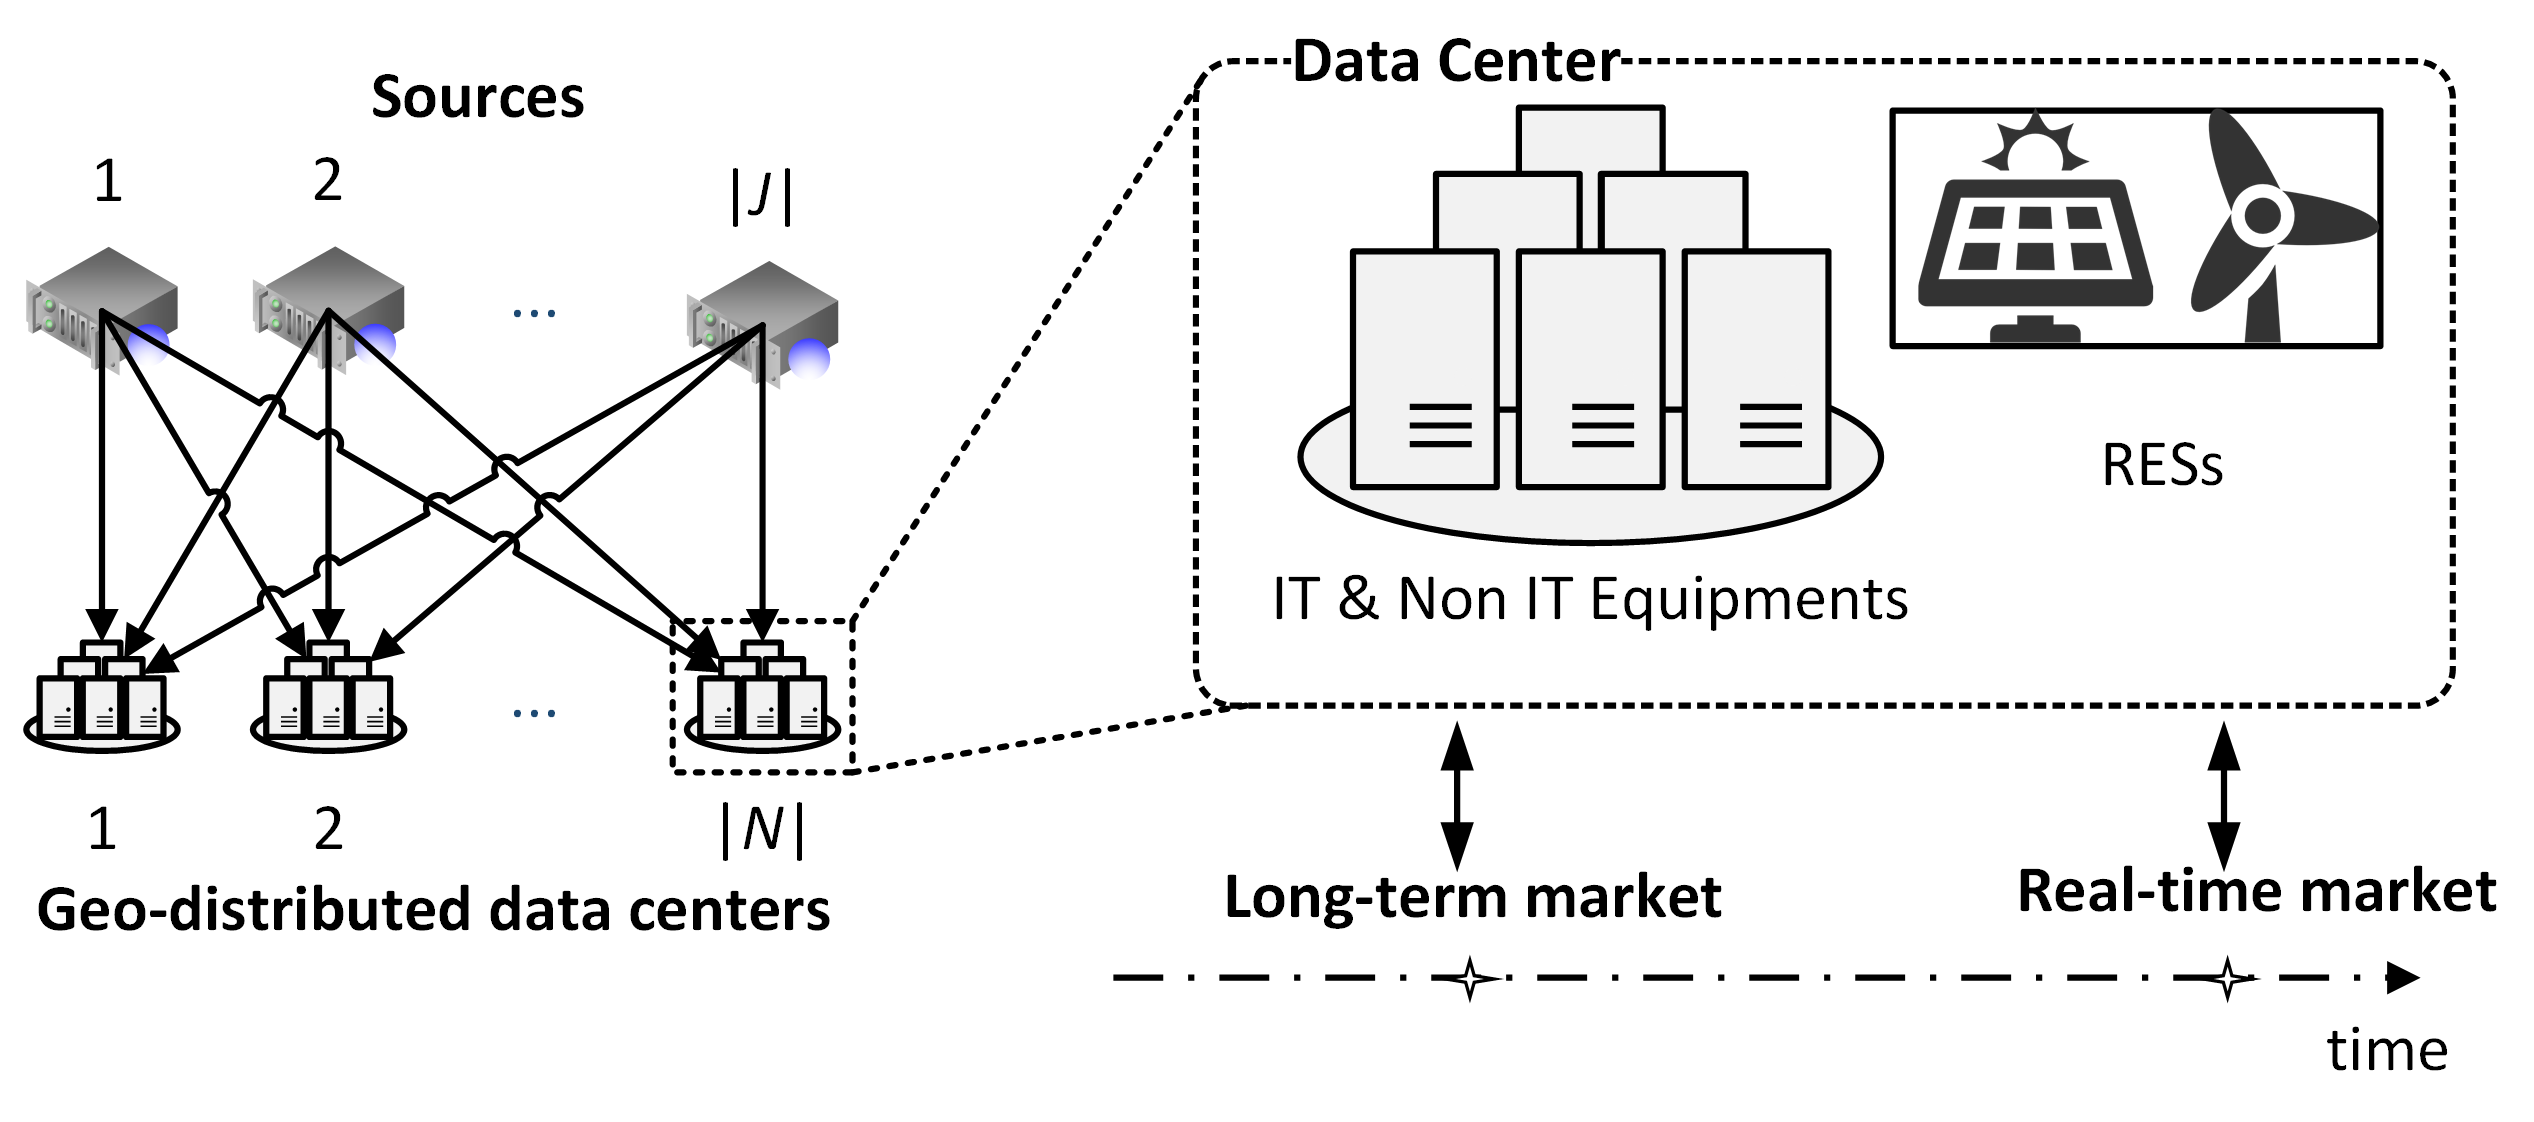
\includegraphics[width=1.0\linewidth]{figs/MultipleDataCenter}
	\vspace{-0.8cm}
	\caption{Geo-distributed data centers in long-term and real-time markets.}
	\label{fig:MultipleDataCenter}
	\vspace{-0.3cm}
\end{figure}

\textbf{Geo-distributed data centers.} We consider a set $N$ of geo-distributed data centers serving workload demands from a set $J$ of sources as illustrated in Figure \ref{fig:MultipleDataCenter}. The workload demand from each source is split between the $|N|$ data centers. Here, a source can represent the aggregate demand from a group of local users, such as users of a particular city, ISP, or geographical region. Each data center has access to renewable energy sources. Further, each data center participates in a (local) long-term electricity market and a (local) real-time electricity market. In other words, each data center $i$ can buy electricity ahead of time in its long-term market, and can also buy additional electricity in its real-time market if necessary. %Note that different data centers may buy from different markets that are locally available to them.

\textbf{Energy procurement system (EPS)}. Our proposed energy
procurement system for geo-distributed data centers is depicted in
Figure \ref{fig:SystemArchitecture}. There are three main components,
namely, the long-term forecaster, the energy procurement
(EP) in long-term markets and the geographical load balancing (GLB). The long-term forecaster provides the forecasted
information for the energy procurement. The forecasted information
includes the predicted values and the prediction error distributions
of IT workload, renewable energy generations, and electricity
prices. We design the algorithms for the long-term forecaster in
Section \ref{sec:dataAnalysis}. The EP component procures electricity
for each data center in the corresponding long-term markets (at time
$t = -T_l$) based on the electricity prices in the long-term markets
and \emph{forecasts} of real-time prices, workload, and renewable
generation. The GLB component (at time $t = 0$) distributes (routes)
the realized workload from sources to data centers, provisions the
required computing capacity at each data center, and procures
additional electricity as needed in the real-time markets.

\textbf{Data center}. Let $M_i$ denote the number of servers in data
center $i$. The number of active servers at real-time (time $t=0$) is
denoted by $m_i,$ which is a control parameter. In practice, there can
be more than a hundred thousand servers in a single data center. Thus,
in our mathematical modeling, we treat $m_i$ as a real number
satisfying $0 \leq m_i \leq M_i.$

\begin{figure}[!t]
	\centering
	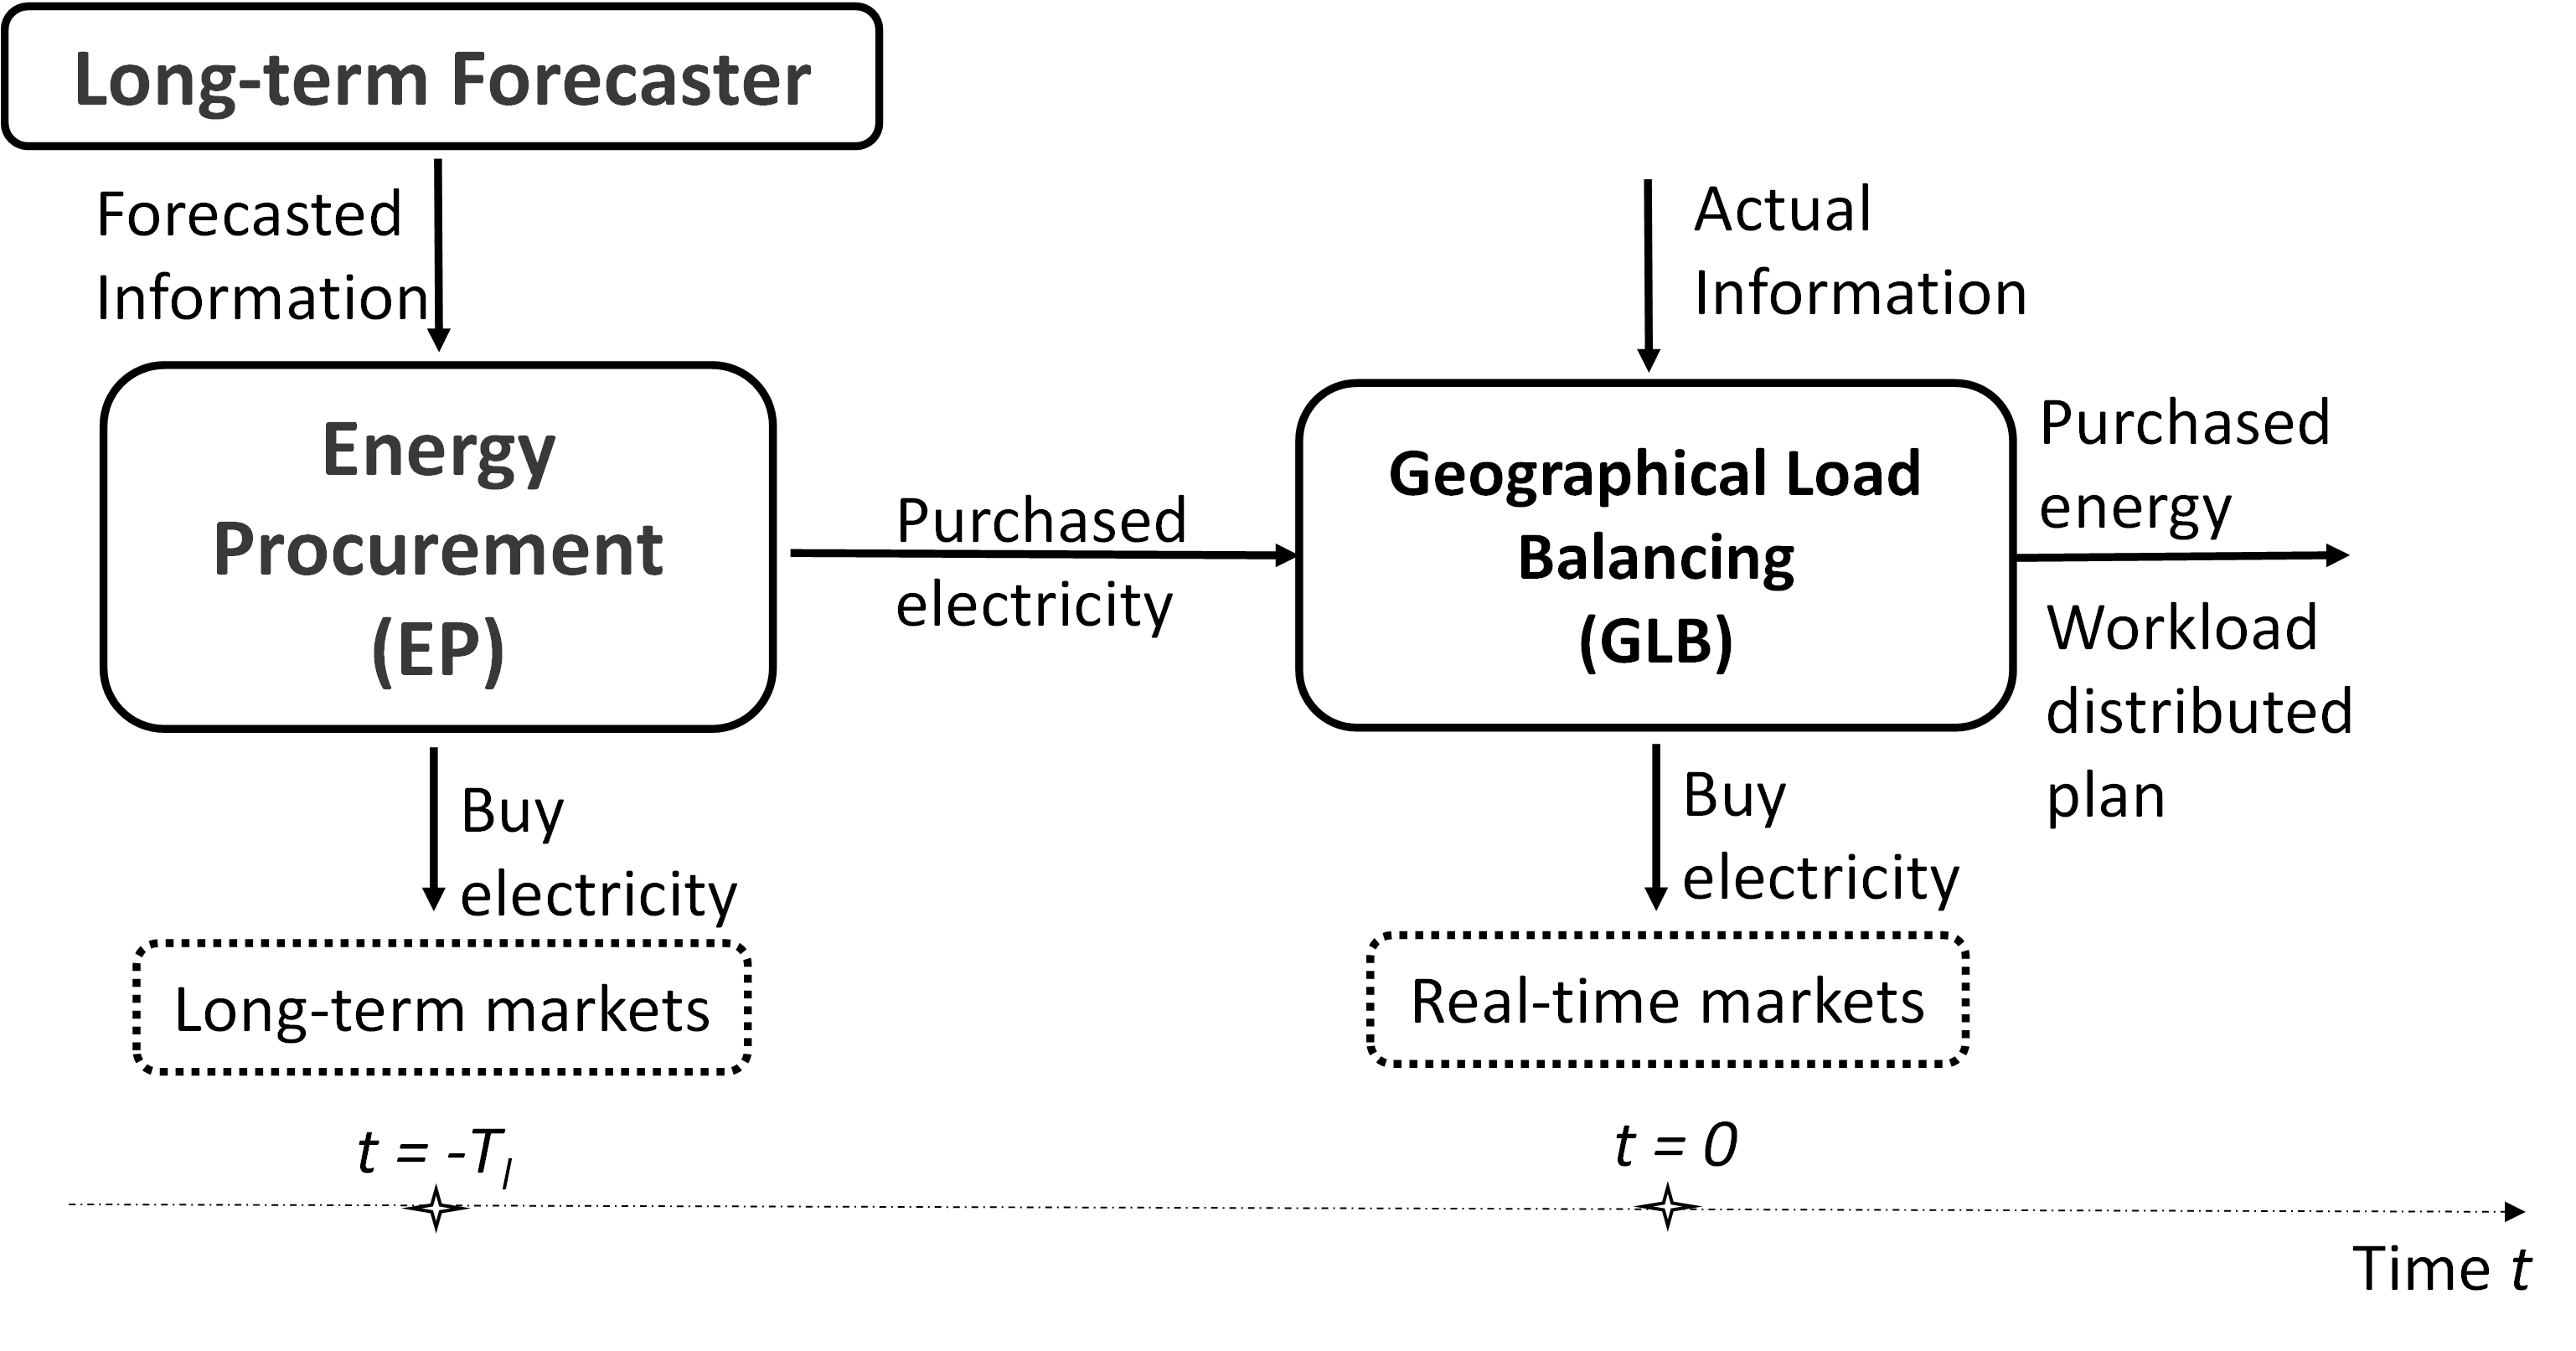
\includegraphics[width=1.0\linewidth]{figs/SystemArchitecture}
	\vspace{-0.8cm}
	\caption{Energy Procurement System (EPS) Architecture for geo-distributed data centers.}
	\label{fig:SystemArchitecture}
	\vspace{-0.3cm}
\end{figure}

At time $t = 0,$ the power consumption of data center $i$ is denoted
by $d^r_i.$ In general, the power consumption of data center $i$ is
dependent on the number of active servers $m_i$ and the workload
arrival
$\lambda_i$. %Let $d^r_i = O_i(m_i, \lambda_i),$ where the power consumption function $O_i(\cdot)$ is non-decreasing in $m_i$ and $\lambda_i$.
For simplicity, we assume that $d^r_i = m_i$, which implies that the
power consumption is proportional to the number of active servers, and
is independent of the workload $\lambda_i$.\footnote{The
  proportionality constant relating the number of active servers and
  the power consumption is taken to be 1 without loss of
  generality. Also, our analysis can be easily generalised to the case
  $d^r_i = O_i(m_i, \lambda_i),$ where the function $O_i$ is
  continuously differentiable, convex, and non-decreasing in each
  coordinate.} %This model is can be applied to other cases, such as
               %the linear power consumption model
               %\cite{rao2011hedging,liu2011greening,
               %liu2012renewable}.


\textbf{Workload}. Workload demand from source $j$ in real-time ($t = 0$) is denoted as $L^r_j.$ We assume that the exact realization of the random vector $\Vector{L}^r = (L^r_j,j \in J)$ is known to the cloud provider at time $t = 0,$ and is an input to GLB. Let $\lambda_{ij}$ denote the distributed workload arrival from source~$j$ to data center $i$ at time $t = 0$ (set by GLB). Thus,
\begin{eqnarray*}
	\label{eq:constraintWorkload1}
	L^r_j = \sum_{i\in N}^{}\lambda_{ij}  & \quad (j\in J), \\
	\label{eq:constraintWorkload2}
	\lambda_i = \sum_{j\in J}^{}\lambda_{ij} & \quad (i \in N).
\end{eqnarray*}

\textbf{Renewable energy}. Data centers can utilize their integrated RESs. Let $w^r_i$ denote the renewable energy generation at data center $i$ in real-time ($t=0$). We assume that the exact realization of the random vector $\Vector{w}^r = (w^r_i,i \in N)$ is known at time $t = 0,$ and is an input to GLB. 
%Moreover, we assume that $w^r_i$ is a continuous random variable for each $i \in N.$

%\david{use "at time $t=0$" or "in real-time ($t=0$)"}

\textbf{Electricity price}. For each data center, the cloud provider can purchase electricity at time $t=-T_l$ in the local long-term market and then purchase any additional electricity needed in the local real-time market at time $t = 0.$ For data center~$i,$ let $p^{l}_i$ denote the long-term price for 1 unit of electricity, and $p^{r}_i$ denote the real-time price for 1 unit of electricity. We assume that $\Vector{p}^l = (p^l_i,i \in N)$ is fixed (or equivalently, is known at the time of the long-term procurement), and $\Vector{p}^r= (p^r_i, i \in N)$ is a random vector whose exact value is known is known at time $t = 0$ and is an input to GLB.

Note that the real-time workload $\Vector{L}^r,$ the real-time
renewable generation $\Vector{w}^r,$ and the real-time electricity
prices $\Vector{p}^r$ are unknown at the time of the long-term
procurement by the EP component, but are known at the time of
operation of the GLB component. We assume that the random vector
$(\Vector{L}^r,\Vector{w}^r,\Vector{p}^r)$ is jointly continuous. In
addition, all the $w^r_i$, $L^r_j$, and $p^r_i$ are assumed to be
bounded random variables.
% $\Exp{w^r_i} < \infty ,\Exp{p^r_i} < \infty$ and $\Exp{L^r_j} < \infty$.

% From the point of view of long-term markets, all the variables in
% real-time are random variables. Hence, workload $L^r_j$, renewable
% energy generation $w^r_i$, and electricity price $p^r_i$ are the
% random variables at time $t=-T_l$. Naturally, they are bounded by
% finite numbers.

\subsection{Cost model}


The total cost of operating geo-distributed data centers in composed of a delay cost and an energy cost. The delay cost is the monetary cost incurred due to the delay in processing the arriving workload. The energy cost is the total electricity bill from the long-term and real-time markets.

\todo{Generalize the delay cost function}

\delete{\textbf{Delay cost}. The delay cost represents the monetary cost
	incurred due to the delay experienced by the sources. We model the
	delay cost $h_{ij}(m_i, \lambda_{i})$ of routing and processing each
	unit of workload from source $j$ to data center $i$ as follows.
}
\begin{eqnarray}
%\label{eq:delaycost}
h_{ij}(m_i, \lambda_{i}) = \beta \bigg (\frac{1}{\mu_i - \lambda_i/m_i} + \pi_{ij}  \bigg ) & \quad (\lambda_i < m_i \mu_i)
\end{eqnarray}
\delete{Here, the parameter $\beta$ weighs the delay
relative to the energy cost. The first term above
captures queuing delay at delay center $i,$ which is based on the
well-known mean delay formula for the M/GI/1 processor sharing queue;
$\mu_i$ is the service rate of servers in data center $i.$ The second
term captures the network delay from source $j$ to data center $i.$
Note that for stability, we need that $\lambda_i < m_i \mu_i.$ Our
delay cost model assumes a linear relationship between delay and its
associated monetary cost, as is suggested in
\cite{Beheshti2012PerformanceImpact}.}

\new{
\textbf{Delay cost}. We consider two delay components, which are network delay and queuing delay. The network delay $\pi_{ij}$ captures the delay that propagates the workload $\lambda_{ij}$ from source $j$ to data center $i$. The queuing delay  $g_i(m_i,\lambda_i)$ denotes the delay at data center $i$ to process its arrival workload $\lambda_i$. We assume that $g_i$ is strictly decreasing
in $m_i$, strictly increasing in $\lambda_i$, and strictly convex in both
$d_i$ and $\lambda_i$. For stability, we need that $\lambda_i < m_i \mu _i$.
Here, $\mu _i$ is the service rate of a server in data center $i$.
Thus, we define $h_{ij}(m_i, \lambda_{i}) = \infty$ for $\lambda_i \geq m_i \mu_i.$}

\new{
	We model the delay cost $h_{ij}(m_i,\lambda_i)$ of routing and processing each unit of workload from source $j$ to data center $i$ as follows.
}
\begin{eqnarray}
\label{eq:gen_delaycost}  
h_{ij}(m_i, \lambda_{i}) = \beta \big ( g_i(m_i,\lambda_i) + \pi_{ij}  \big ).
\end{eqnarray}
\new{
Here, the parameter $\beta$ weighs the delay
relative to the energy cost. While {\eqref{eq:gen_delaycost}} assumes a linear
relationship between incurred delay and the associated monetary cost
(as is suggested in {\cite{Beheshti2012PerformanceImpact}}), our model
allows for even a non-linear (convex) relationship between delay and
its monetary cost to the cloud provider. The delay cost of transmitting workload {$\lambda_{ij}$} from source $j$ to data center {$i$} is computed as $\lambda_{ij}h_{ij}(m_i,\lambda_i)$. We assume that
$\lambda_{ij}h_{ij}(m_i, \lambda_{i})$ is continuously differentiable, convex,
strictly decreasing in $m_i,$ and strictly increasing in $\lambda_i.$
}


\delete{We denote the the delay cost of routing and processing each unit of
	the workload from source $j$ to data center $i$ by $h_{ij}(m_i,
	\lambda_{i}).$ For stability, we need that $\lambda_i < m_i \mu_i,$
	where $\mu_i$ is the speed of each server of data center~$i.$ Thus, we
	define $h_{ij}(m_i, \lambda_{i}) = \infty$ for $\lambda_i \geq m_i
	\mu_i.$ For $0 \leq \lambda_i < m_i \mu_i,$ we assume that
	$h_{ij}(m_i, \lambda_{i})$ is continuously differentiable, convex,
	strictly decreasing in $m_i,$ and strictly increasing in $\lambda_i.$}

A specific instance of the delay cost function $h_{ij}$ that satisfies
the above assumptions, and which we use in our \new{numerical}
evaluations, is
\begin{eqnarray}
\label{eq:delaycost}
%h_{ij}(m_i, \lambda_{i}) = \beta \bigg (\frac{1}{\mu_i - \lambda_i/m_i} + \pi_{ij}  \bigg ) & \quad (\lambda_i < m_i \mu_i),
h_{ij}(m_i, \lambda_{i}) = \beta \bigg (\frac{1}{\mu_i - \lambda_i/m_i} + \pi_{ij}  \bigg ) & \quad (\lambda_i < m_i\mu_i),
\end{eqnarray}
\new{where the first term $\frac{1}{\mu_i - \lambda_i/m_i}$ above
captures queuing delay at delay center $i,$ which is based on the
well-known mean delay formula for the M/GI/1 processor sharing
queue.} \delete{The second term captures the network delay from source $j$ to
data center $i.$ While {\eqref{eq:delaycost}} assumes a linear
relationship between incurred delay and the associated monetary cost
(as is suggested in \cite{Beheshti2012PerformanceImpact}), our model
allowes for even a non-linear (convex) relationship between delay and
its monetary cost to the cloud provider.}

%%JK -- I don't think this generalization is correct.

%%be proportional to a certain range of delay
%\cite{Beheshti2012PerformanceImpact}.

%Here, $\mu_i$ is the service rate of servers in data
%center $i.$ We require that
%\begin{eqnarray*}
%	\lambda_i \leq m_i \mu_i & \quad (i\in N).
%\end{eqnarray*}


% There could be several ways to model the delay cost based on the
% responsive time. For instance, the lost revenue can be proportional
% to a certain range of delay \cite{Beheshti2012PerformanceImpact}. We
% assume that the delay cost of routing and processing each unit of
% the workload from source $j$ to data center $i,$ denoted
% $h_{ij}(m_i, \lambda_{i}),$ is jointly convex over $(m_i,
% \lambda_{i}).$



% Thus, we model the delay cost $h_{ij}(m_i, \lambda_{i})$ of routing
% and processing each unit of the workload from source $j$ to data
% center $i$ as follows.  We consider delay $h_{ij}(m_i, \lambda_{i})$
% in real-time when routing and processing each unit of workload from
% sources $j$ to data center $i$. We assume that $h_{ij}(m_i,
% \lambda_{i})$ is convex, increasing in $m_i$, and decreasing in
% $\lambda_{i}$. In particular, we use the following delay cost model
% for further analysis and evaluation.

%$p^r_i$ has to be in an acceptable range $ [\underbar{p}^{r},\bar{p^{r}}] $. Let $f_{p^{r}}(\cdot)$ is the probability density function of the real-time prices. $f_{p^{r}}(\cdot)$ is assumed to be continuous over $ (\underbar{p}^{r},\bar{p^{r}}) $.

\desc{Energy cost}

\textbf{Energy cost}. Let $q^l_i$ and ${q}_i^r$ respectively denote the amount of electricity purchased in the long-term market and the real-time market by data center $i.$ Here, we require that sufficient electricity is procured to process the workload routed to each data center as
$$q^r_i + w^r_i + q^l_i \geq d^r_i \quad (i \in N).$$
%The the amount of long-term energy $q^l_i$ and the amount of real-time energy $q^r_i$ are related as
%\begin{align}
%q^r_i &= [m_i - w^r_i - q^l_i]_+,
%\end{align}
%where $[x]_+$ is equal to the maximum of $\{x,0\}$. Hence, $q^r_i \geq 0$ and $q^r_i \geq  m_i - w^r_i - q^l_i$.
%JK -- I think these deductions should come later.
The electricity bills of data center $i$ in the long-term market and the real-time market are respectively computed as
\begin{align*}
	R^l_i(q^l_i) &= p^l_i q^l_i & i\in N, \\
	R^r_i(q^r_i) &= {p}_i^r q^r_i & i \in N.
\end{align*}
%where $R^l_i(q^l_i)$ is the long-term electricity cost and $R^r_i(q^r_i)$ is the real-time electricity cost.

% \begin{eqnarray}
% \label{eq:totalCost}
% F(\Vector{q}^l,\Vector{m}, \Vector{\lambda}, \Vector{p}^r) = \sum_{i\in N}^{} R^l_i(q^l_i) + F^r(\Vector{q}^l,\Vector{p}^r,\Vector{L}^r,\Vector{w}^r)
% \end{eqnarray}
% where $\Vector{q}^l,\Vector{m},$, $\Vector{\lambda}$, and $\Vector{p}^r$ are the vectors of $\{q^l_i\}_{i \in N}, \{m_i\}_{i \in N},$, $\{\lambda_{ij}\}_{i \in N, j \in J}$, and $\{p^r_i\}_{i\in N}$ respectively. The real-time cost objective computed as
% \begin{equation}
% \label{eq:rt-obj2}
% F^r(\Vector{q}^l,\Vector{p}^r,\Vector{L}^r,\Vector{w}^r) =  \sum_{i \in N}^{} R_i^r(q^r_i)+ \beta\sum_{i,j \in N,J} \lambda_{ij}h_{ij}(m_i,\lambda_i),
% \end{equation}
% where $\beta$ weighs the importance of the delay cost.

% We notice that working out the total cost \eqref{eq:totalCost} is extremely challenging because there are bidirectional influence between two different time-scales, i.e., long term and real-time. In chronological order, our energy procurement system first computes the best long-term procurement, $\Vector{q}^l$. However, the system has to consider its impact on real-time markets which are very uncertain and vise versa. It is because our energy procurement system also minimizes the total cost $F^r(\Vector{q}^l,\Vector{m},\boldsymbol{\lambda} , \Vector{p}^r, \Vector{w}^r)$ in real-time, denoted as 
% $$\min_{} F^r(\Vector{q}^l,\Vector{m},\Vector{\lambda},\Vector{p}^r,\Vector{w}^r).$$

\subsection{Formulation of optimal energy procurement in multi-timescale markets}

In this section, we describe the optimization formulation for optimal energy procurement. Recall that the total cost of operating geo-distributed data centers in our two-timescale market setting is the sum of the energy cost and the delay cost, given by $$F = \sum_{i\in N}^{} R^l_i(q^l_i) + \sum_{i \in N}^{} R_i^r(q^r_i)+ \sum_{i \in N,j \in J} \lambda_{ij}h_{ij}(m_i,\lambda_i).$$
We seek to minimize $\Exp{F}$ subject to the aforementioned constraints. Note that this optimization is performed on two timescales, with different sets of information available at each. The EP component optimizes the long-term procurements $\Vector{q}^l = (q^l_i, i\in N)$ given only distributional information of the real-time workload $\Vector{L}^r,$
the real-time renewable generation $\Vector{w}^r,$ and the real-time electricity prices $\Vector{p}^r.$ The GLB component optimizes the workload routing $\Vector{\lambda} = (\lambda_{ij},i\in N,j \in J),$ the number of active servers $\Vector{m} = (m_i,i \in N)$ at the data centers, and the real-time procurements $\Vector{q}^r = (q^r_i,i \in
N)$ given the prior long-term procurements $\Vector{q}^l,$ and the exact realization of $(\Vector{p}^r,\Vector{L}^r,\Vector{w}^r).$
Below, we first formalize the real-time optimization, followed by the long-term optimization.

\textbf{Geographical load balancing in real-time markets}. 

Note that in real-time, GLB optimizes the real-time procurements
$\Vector{q}^r$, the numbers of active servers $\Vector{m}$, and the workload routing $\Vector{\lambda},$ given the long-term procurements $\Vector{q}^l$ and the realization of the random vector $(\Vector{p}^r,\Vector{L}^r,\Vector{w}^r).$ The total cost as seen by GLB is $$F^r(\Vector{q}^r, \Vector{m},\Vector{\lambda},\Vector{p}^r)
:= \sum_{i \in N}^{} R_i^r(q^r_i)+ \sum_{i\in N, j \in J}
\lambda_{ij}h_{ij}(m_i,\lambda_i).$$ Thus, the real-time optimization is defined as follows.

\vspace{0.1in}
\begin{subequations}
	\begin{align}
	\text{\bf{GLB-RT}: } &  \min_{\Vector{m}, \Vector{\lambda}, \Vector{q}^r} F^r(\Vector{q}^r, \Vector{m},\Vector{\lambda},\Vector{p}^r) \nonumber \\
	\mbox{s.t. } \nonumber \\
	\label{eq:GLB-RT_c1}
	&\lambda_{ij} \geq 0  \quad \forall i \in N,j \in J \\
	&\sum_{i\in N}^{} \lambda_{ij} = L^r_j \quad \forall j \in J \\
	\label{eq:GLB-RT_c}
	% &\sum_{j\in J}^{} \lambda_{ij} = \lambda_i &\forall i \in N \\
	&\lambda_i \leq m_i \mu_i,   \quad \forall i \in N\\
	&0 \leq m_i \leq M_i \quad \forall i \in N \\
	\label{eq:GLB-RT_c2}
	&q^r_i \geq 0, \quad \forall i \in N \\
	\label{eq:GLB-RT_c3}
	& m_i - q^r_i - w^r_i \leq q^l_i \quad \forall i \in N
	\end{align}
\end{subequations}
\vspace{0.1in}

Since $p^r_i \geq 0,$ it easily follows that any solution of the above optimization problem satisfies $q^r_i =[m_i - w^r_i - q^l_i]_+,$ where $[x]_+ := \min\{0,x\}.$ Thus, the real-time objective can be re-written as 
\begin{equation}
\label{eq:rt-obj2}
\begin{array}{rl}
&\tilde{F}^r(\Vector{q}^l,\Vector{m},\Vector{\lambda},\Vector{p}^r,\Vector{w}^r) = \sum_{i \in N} p^r_i [m_i - w^r_i - q^l_i]_+ \\
& \qquad+ \sum_{i\in N, j \in J}
\lambda_{ij}h_{ij}(m_i,\lambda_i).    
\end{array}
\end{equation}
With this notation, GLB-RT can be equivalently expressed as follows.
\begin{subequations}
	\begin{align*}
	& \min_{\Vector{m}, \Vector{\lambda}} \tilde{F}^r(\Vector{q}^l,\Vector{m},\Vector{\lambda},\Vector{p}^r,\Vector{w}^r) \\
	\mbox{s.t. } \nonumber \\
	&(\Vector{m},\Vector{\lambda}) \in C(L^r).
	\end{align*}
\end{subequations}
Here, the convex compact set $C(L^r)$ is defined by the constraints
\eqref{eq:GLB-RT_c1}--\eqref{eq:GLB-RT_c2}.
%%to be moved to the appendix where this will be used.


GLB-RT problem is a convex optimization problem and hence can be solved efficiently using standard techniques \cite{boyd2004convex}. For instance, CVX (Matlab Software for Disciplined Convex Programming) tool \cite{grant2008cvx} can be used to solve GLB-RT. 
%In Section~\ref{sec:char_glb-rt}, we prove several interesting properties of the optimal solutions of GLB-RT.


\textbf{Energy procurement in long-term markets}. At time $t=-T_l$,
the cloud provider purchases electricity $\Vector{q}^l$ in
long-term markets that will be used at real-time. Note that
optimization of the long-term procurements has to be performed based
only on distributional information for the random vector
$(\Vector{p}^r,\Vector{L}^r,\Vector{w}^r),$ and subject to the
real-time optimization that will be subsequently performed based on
the realization of the random vector
$(\Vector{p}^r,\Vector{L}^r,\Vector{w}^r).$ 

Let us denote the optimal value of the optimization GLB-RT by
$F^{*r}(\Vector{q}^l,\Vector{p}^r, \Vector{L}^r, \Vector{w}^r).$ The
long-term objective is thus defined as $$F^l(\Vector{q}^l) :=
\sum_{i\in N} R^l_i(q^l_i) + \Exp{F^{*r}(\Vector{q}^l,\Vector{p}^r,
	\Vector{L}^r, \Vector{w}^r)}.$$ Note that the above expectation is
with respect to the random vector
$(\Vector{p}^r,\Vector{L}^r,\Vector{w}^r).$ The long-term optimization
problem is then given by:
\begin{subequations}
	\begin{align*}
	\text{\bf{EP-LT}: }  & \min F^l(\Vector{q}^l) \\
	\mbox{subject to } \nonumber \\
	& \Vector{q}^l \in \mathbb{R}^N_+.
	\end{align*}
\end{subequations}

The above optimization is more challenging than GLB-RT. In
Section~\ref{sec:char_ep-lt}, we prove that EP-LT is a convex
optimization and characterize the gradient of the objective
function. These results are then used to arrive at a provably optimal stochastic gradient algorithm in Section~\ref{sec:AlgorithmDesign}.

\section{\diff{Characterizing the Optima}}
\label{sec:characterizingOptima}

In this section, we collect useful properties of the optimizations
EP-LT and GLB-RT. These are important for understanding the behavior
of the energy procurement system, and also for proving convergence of
the stochastic gradient algorithm for EP-LT in
Section~\ref{sec:AlgorithmDesign}.


%\subsection{Characterizations of EP-LT}

\label{sec:char_ep-lt}

Our first result is that EP-LT is indeed a convex optimization, which
suggests that EP-LT is a tractable optimization.

% One may worry that EP-LT may not be convex, which results in hardly
% finding the global optimal solution in multidimensional search
% space. We claim that EP-LT is surprisingly convex as

\begin{theorem}
	\label{theorem:LT-Convexity}
	$F^l(\textbf{q}^l)$ is convex over $\textbf{q}^l \in \mathbb{R}^N_+.$
\end{theorem}
We provide the proof of Theorem~\ref{theorem:LT-Convexity} in Appendix~\reference{proof:convexity}{A.1 of our technical report \cite{le2016SoCCTechnicalReport}}. Next, we characterize the gradient of the EP-LT objective function as
follows.

\begin{theorem}
	\label{theorem:lt_gradient}
	The gradient of $F^l(\cdot)$ is characterised as follows.
	\begin{align*}
	\frac{\partial F^l(\textbf{q}^l)} {\partial q^l_i} &= p^l_i +
	\mathbb{E} \bigg[ \frac{\partial F^{*r}(\textbf{q}^l,\textbf{p}^r,\textbf{L}^r,\textbf{w}^r)}  {\partial q^l_i} \bigg] \\
	&=p^l_i -\mathbb{E}
	\left[\varrho_i(\textbf{q}^l,\textbf{p}^r,\textbf{L}^r,\textbf{w}^r)
	\right],
	\end{align*}    
	where $\varrho_i(\textbf{q}^l,\textbf{p}^r,\textbf{L}^r,\textbf{w}^r)$
	is the unique Lagrange multiplier of GLB-RT corresponding to the
	constraint \eqref{eq:GLB-RT_c3}.
\end{theorem}


Note that the first equality in the theorem statement asserts that the
order of an expectation and a partial derivative can be
interchanged. The second equality relates the partial derivative of
$F^{*r}$ with respect to $q^l_i$ to a certain Lagrange multiplier of
GLB-RT. We provide the proof of Theorem~\ref{theorem:lt_gradient} in
Appendix~\reference{proof:lt_grad}{A.2 of our technical report \cite{le2016SoCCTechnicalReport}}.

We note that Theorem~\ref{theorem:lt_gradient} does not enable us to
compute the gradient of the $F^l(\cdot)$ exactly. Indeed, the
expectation of the Lagrange multiplier $\varrho_i$ with respect to
$(\Vector{p}^r,\Vector{L}^r,\Vector{w}^r)$ would in general be
analytically intractable. However, Theorem~\ref{theorem:lt_gradient}
does enable a noisy estimation of the gradient of the $F^l(\cdot)$ via
Monte Carlo simulation as follows. Suppose we simulate a finite
number, say $\mathbb{S},$ of samples from the distribution of
$(\Vector{p}^r,\Vector{L}^r,\Vector{w}^r).$ In practice, we can obtain
these samples by using real-world traces as is done in Section
\new{\ref{sec:caseStudy}}. For each sample, the Lagrange multipliers
$(\varrho_i, i \in N)$ can be computed efficiently by solving
GLB-RT. By averaging the $\mathbb{S}$ instances of $(\varrho_i, i \in
N)$ thus obtained, we get an unbiased estimate of the gradient of
$F^l(\cdot).$ This, in turn, enables us to solve EP-LT using a
stochastic gradient descent method; details follow in
Section~\ref{sec:AlgorithmDesign}.


%\subsection{Characterizations of GLB-RT}
%\label{sec:char_glb-rt}
%\new{
As there are two timescales in optimization, it is critical to investigate how EP-LT affects the operation of geographical load balancing in real-time. We start by answering the following question: how does the long-term procurement $\Vector{q}^l$ impact the power consumption $d^r_i$ in data center $i$? Formally, we have the following intuitive result:
\begin{lemma}    
	\label{theorem:RealTimeOptimalDemand}
	At any data center $i$, an optimal solution always utilizes the long term energy procurement $q^l_i$ and renewable generation $w^r_i$ as much as possible. It is simply represented by
	\begin{eqnarray}         
	\begin{cases} 
	m_i \geq w^r_i+q^l_i  &\mbox{if  } w^r_i + q^l_i < M_i \\ 
	m_i = M_i & \mbox{if  } w^r_i + q^l_i \geq M_i. 
	\end{cases}
	\end{eqnarray}
\end{lemma}
\begin{proof} Appendix~\reference{proof:RealTimeOptimalDemand}{A.3 of our technical report \cite{le2016SoCCTechnicalReport}}.
\end{proof}
The above lemma states that a data center $i$ uses up the reserved
electricity, including free renewable energy and pre-purchased
electricity, because doing so reduces the queueing delay.


%In addition, our problem preserves two other properties of GLB along the lines of
%\cite{liu2011greening} (which considers GLB without the preceding
%long-term procurement): the \textit{uniqueness} of optimal solution and the
%\textit{sparsity of routing}.
%% It turns out that both properties are preserved in our system.
%The uniqueness property states that the service arrival rate at any
%data center $i$, $\lambda_i/m_i$, is unique among all optimal
%solutions. The sparsity property asserts that the number of routing table entries used in
%the simplest optimal solution is less than or equal to $|N|+|J|-1$, which
%is much smaller than the maximum number of entries, i.e., $|N|\times|J|$. 
%Such sparsity is naturally desirable in practice. We omit the proof and readers can refer to
%the proof of Theorems~2 and~3 in \cite{liu2011greening} for more details.


%To begin, it is easy to see that GLB-RT has at least one optimal solution. Although the optimal solution is generally not unique, there are natural aggregate quantities that are unique over the set of optimal solutions, which is a convex set. The optimal solutions preserve the uniqueness and sparsity properties of GLB as in existing works \cite{liu2011greening}. The uniqueness of optimal solutions say that the server arrival rate, $\bar{\lambda}_i = \lambda_i/m_i$, is common across all optimal solutions. It would be impractical if the optimal solutions of GLB-RT required that requests from each source were divided up among all of the data centers. In general, each $\lambda_{ij}$ could be nonzero in an optimal solution, yielding flows of requests from all sources to all data centers. In practice, this would lead to significant scaling issues. The sparsity of optimal solutions allows cloud providers to transform any optimal solution into a practically optimal solution. 




%Implicitly, there is a trade-off between energy cost and queueing delay cost.
\section{Predictability Analysis}
\label{sec:dataAnalysis}

\begin{figure*}[!ht]
	\centering
%	\vspace{-0.3cm}
	\subfloat[PV generation]{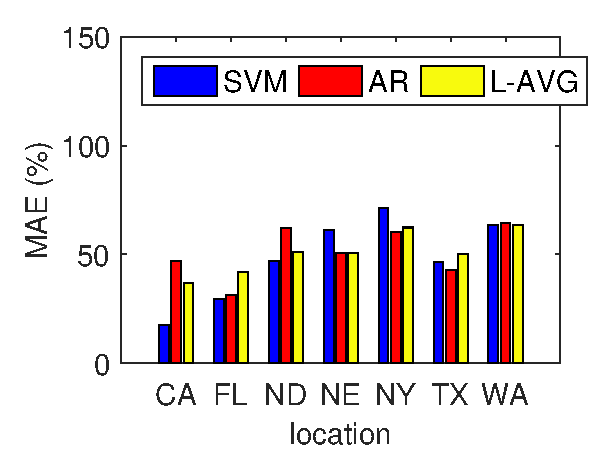
\includegraphics[width=.24\linewidth]{figs/svm_vs_ar_vs_avg_solar}}
	\subfloat[Wind generation]{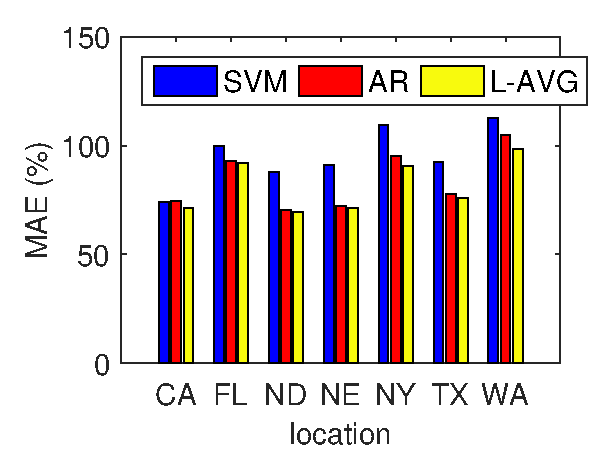
\includegraphics[width=.24\linewidth]{figs/svm_vs_ar_vs_avg_wind}}
	\subfloat[Electricity price]{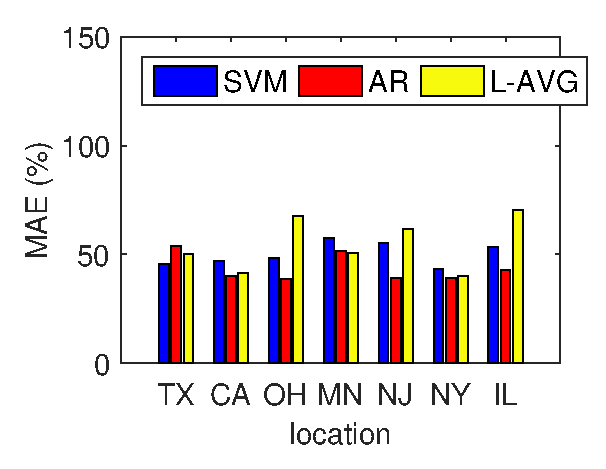
\includegraphics[width=.24\linewidth]{figs/svm_vs_ar_vs_avg_price}}
	\subfloat[Workload]{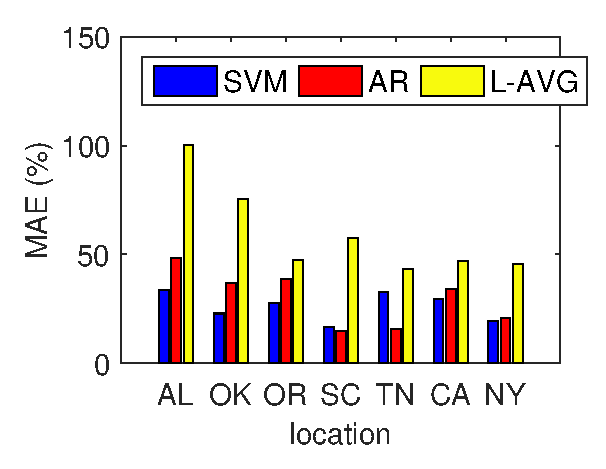
\includegraphics[width=.24\linewidth]{figs/svm_vs_ar_vs_avg_workload}}
	\caption{Comparisons of SVM, AR and L-AVG. The codes of US states are California (CA), Florida (FL), North Dakota (ND), Nebraska (NE), New York (NY), Texas (TX), Washington (WA), Ohio (OH), Minnesota (MN), New Jersey (NJ), Illinois (IL), Alabama (AL), Georgia (GA), Oklahoma (OK), South Carolina (SC), Virginia (VA), and Tennessee (TN).}
	\label{fig:CompareARandAVG}
%	\vspace{-0.5cm}
\end{figure*}

\diff{In this section, we study the long-term predictability of metrics
critical to our procurement systems for multi-timescale markets;
namely, workload, renewable generation, and real-time electricity
price. 
We design two long-term prediction methods, and analyse the prediction 
errors associated with each metric using real-world traces.
Our analysis also provides several insights into the nature of the
\emph{distributions} of these metrics.}

% The main purpose of our analysis is used as inputs for our proposed
% procurement systems and provide some insights into the long-term
% prediction errors associated with each metric.
For our study, we collected 3-year real-world traces of photovoltaic
(PV) generation, wind generation, and electricity prices for 20 states
of the US. The 3-year PV and wind generation data were downloaded
using the System Advisor Model (SAM) software, developed by the
National Renewable Energy Laboratory (NREL) \cite{nrel2010SAM}. The
3-year electricity price data are from different regional transmission
operators (RTOs) in the US, i.e., PJM, MISO, CAISO, ISONE, and NYSIO
\cite{qureshi2009cutting}. In addition, we collected 2-month workload
data for the same 20 states from Akamai Technologies, which serves
15-30\% of all Web content around the world from hundreds of data
centers around the world \cite{NygrenSS10}.

%In prior literature, prediction methods fall into one of the two categories: statistical methods and physical methods \cite{lei2009review}. The statistical methods or time-series-based methods exploit the correlation of data in the temporal domain to predict the future from the past data. The statistical methods include linear and non-linear regression models \cite{guoyang2005discussion}, Kalman filter \cite{louka2008improvements}, and machine learning techniques \cite{paoli2010forecasting, sfetsos2000univariate}. In the meantime, the physical methods use correlated physical conditions, such as geographical information, weather data, and time, to predict the future \cite{sharma2011predicting}. 

Long-term prediction is challenging for both statistical and physical
prediction methods \cite{lei2009review}. Statistical methods have to
deal with the weak correlation between the past and future
data. Meanwhile, physical methods require the input of physical
features that are often not available for long-term predictions. For
example, long-term weather forecast requires data from many parts of
the world which are only available in some specialized centers. %{\cite{wmoLongTermForecasting}}.
To improve the prediction accuracy,
prediction methods may exploit seasonality, such as annual
patterns. However, the effectiveness of using seasonality depends
heavily on the characteristics of the data.

%In order to design a prediction algorithm, it is necessary to understand the characteristics of the underlying data. Therefore, we first perform periodicity analysis over PV generation, wind generation, electricity prices, and workload respectively and the results are shown in Figure \ref{fig:periodgram}. The highest peaks occur at 24 hours in all the periodograms, which indicates the strong daily patterns of the data. %The behaviors of solar, wind, electricity price, and workload actually exhibit daily patterns. 

%As the long-term forecaster is a part of our energy procurement
%system, it is necessary to design a reliable long-term forecast method
%to produce the inputs for the energy procurement system. 
We design two long-term prediction methods to produce the inputs for
our energy procurement system: An autoregressive (AR) model and a
Support Vector Machine (SVM) model. The motivation for using the AR
method is to capture daily patterns and the correlation between past
and future data. On the other hand, we develop the SVM method to
capture the seasonality of the data.

In particular, our AR model predicts the value $x(day+d\_ah,hr)$ at
hour $hr$ for $d\_ah$ day-ahead based on the past $A$ days as
$x(day+d\_ah,hr) = \sum_{a=0}^{A-1} \omega_a x(day-a,hr) + c.$ The AR
model can obtain the coefficients $\omega_a$ and constant $c$ by
fitting the model to the historical data. We observe that it is not
necessary to pick a large value of $A$ for long-term prediction
because $A=7$ already achieves  competitive
performance. Additionally, $d\_ah$ is set at 30 days for PV
generation, wind generation, and electricity price, and at 1 day for
workload due to the limited length of data.


Our SVM model is designed to capture the seasonality of workload,
renewable generation, and electricity price.
% SVM is well-known as a learning algorithm for classification and
% regression analysis. JK -- not needed, in my opinion
%Similar to the work \cite{sharma2011predicting}, we focus the
%multi-class SVM that aims to estimate a predicted value based on given
%inputs. 
Similar to the work \cite{sharma2011predicting}, we use a multi-class
SVM. The first input to the SVM model is the average of the past $A$
days. The rest of inputs are the seasonality data, i.e., month of
year, day of month, day of week, and hour of day
\cite{deoras2010MatLabForecast}. For electricity generation from PV panels and wind turbines, we use month of year, day of month, and hour of day to
capture their seasonality. Similarly, we use month of year, day of
month, hour of day, and day of week in predicting electricity
prices. Due the limitation of the trace length, only day of week and
hour of day are used as the seasonality inputs for predicting
workload. The prediction window is the same as with the AR method,
i.e., 30 days for solar generation, wind generation, and electricity
prices, and 1 day for workload. The accuracy of SVM depends on the
selection of SVM kernel function and the kernel parameters. For each
set of data, we search for the best kernel function and the best
kernel parameters using LIBSVM, an SVM tool
\cite{chang2011libsvm}. The most suitable kernel function is Radial
Basis Function (RBF) but the kernel parameters differ for each
dataset.



\textbf{Prediction error analysis:} We now analyse the prediction errors under the AR and SVM methods.
%Prediction errors are used as a metric to quantify the performance of AR and SVM methods.
%Let $\hat{L}^r_j$, $\hat{w}^r_i$, and $\hat{p}^r_i$ denote long-term predicted values of renewable generation, workload, and electricity price. Further, let
%\begin{subequations}
%	\label{eq:predictionErrors}
%	\begin{align}
%		\varepsilon_i = {w}^r_i - \hat{w}^r_i, \\
%		\xi_j  = {L}^r_j - \hat{L}^r_j, \\
%		\epsilon_i = {p}^r_i - \hat{p}^r_i,
%	\end{align}
%\end{subequations}
%where $\varepsilon_i$, $\xi_j$, and $\epsilon_i$ are the prediction errors of renewable generation, workload, and electricity prices, respectively. 
We normalize the prediction errors by the average of real values and
show the values in percentage. For instance, a prediction error for PV
generation of 20 (-20) implies that we underestimate (overestimate)
the PV generation by 20\% of the average PV generation.

\desc{Comparison between SVM vs. AR vs. AVG}



We compare AR and SVM with a baseline method, long-term average
(L-AVG) {\cite{sinden2007characteristics}}. L-AVG assumes that the
long-term data has a long-term cycle. For example, PV generation may
have a yearly cycle. L-AVG takes the average of 30 days at the same
time over the past 2 years for PV generation, wind generation, and
electricity price. In particular, the predicted value at hour $hr$ of
day $day$ in $yr$ is computed as $x(yr, day,hr) =
\frac{1}{2}\sum_{y=1}^{2}\frac{1}{30}\sum_{d=15}^{-14}x(yr-y,day-d,hr)
.$ Assuming that user behavior has a weekly pattern, L-AVG takes the
averages of the workload demand at the same time of 7 days in the past
weeks. The mean absolute errors (MAEs) of three methods are
illustrated in Figure \ref{fig:CompareARandAVG}. In general, SVM and
AR do not perform better than L-AVG in predicting solar and wind
generation but they are better than L-AVG in predicting electricity
price, and workload. In predicting PV generation, SVM outperforms
others methods in some states like California that reveal the positive
impact of seasonality. However, some states like Washington (WA) and
New York (NY) having high precipitation can negatively affect the
performance of SVM and AR. Predicting wind generation is the hardest
among the four types of data as the prediction errors are very
large. It is because the wind generation often has very large
variation and fluctuation. On the other hand, SVM and AR are better
than L-AVG in terms of predicting electricity prices. AR is
surprisingly better than SVM in most states except for Texas (TX). The
seasonality in real-time electricity prices is not strong enough to
benefit SVM in long-term prediction. AR and SVM perform very well in
predicting workload compared to L-AVG in short-term. Overall, the
long-term prediction errors are relatively large compared to the mean
of measured data. Figure {\ref{fig:CompareARandAVG}} also highlights
that long prediction errors are dependent on locations, the types of
data, and the prediction methods. %

\begin{figure*}[pbth]
	\centering
%	\vspace{-0.3cm}
	\subfloat[PV generation]{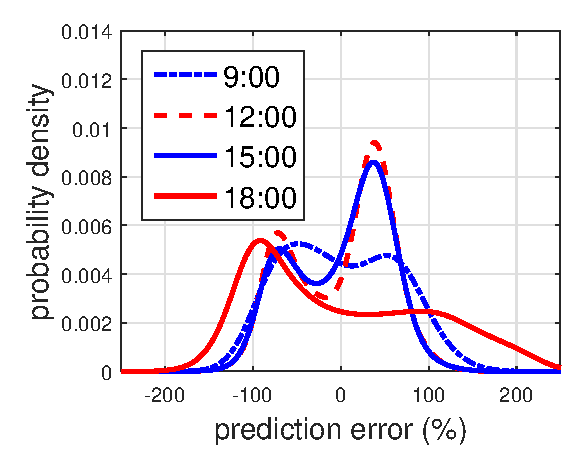
\includegraphics[width=.24\linewidth]{figs/ar_hourly_pdf_error_solar}}
	\subfloat[Wind generation]{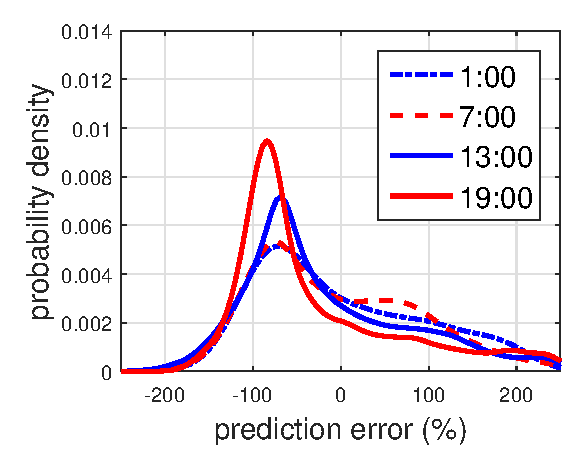
\includegraphics[width=.24\linewidth]{figs/ar_hourly_pdf_error_wind}}
	\subfloat[Electricity price]{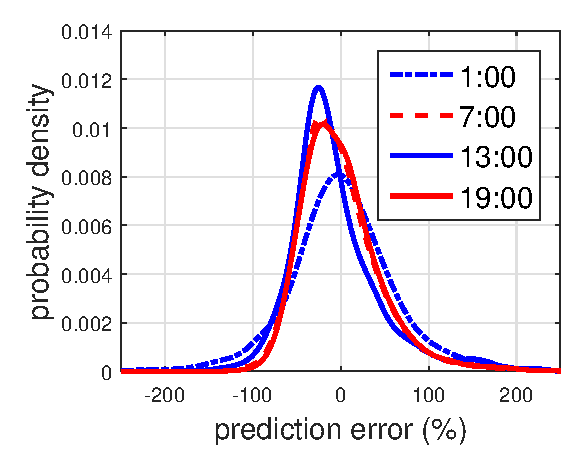
\includegraphics[width=.24\linewidth]{figs/ar_hourly_pdf_error_price}}
	\subfloat[Workload]{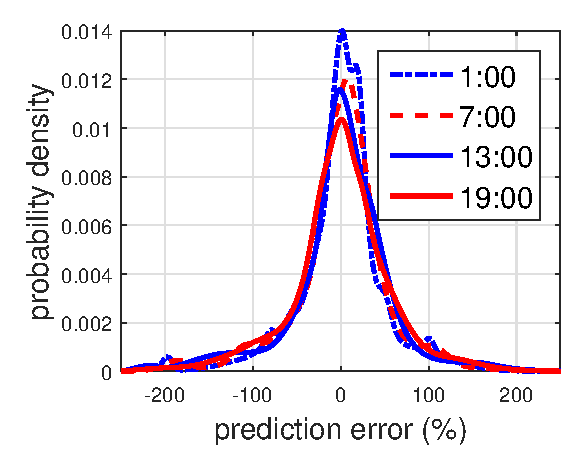
\includegraphics[width=.24\linewidth]{figs/ar_hourly_pdf_error_workload}}	
%	\vspace{-0.2cm}
	\caption{Probability density of prediction errors at different time of the day.}	
	\label{fig:hourlyDistribution}
%	\vspace{-0.4cm}
\end{figure*}

\textbf{What do the distributions of prediction errors look like?} Figure \ref{fig:hourlyDistribution} shows the probability density of the prediction errors at different times in a day of using the AR method. Each line represents the probability density of prediction errors during\delete{ an hour in a day}\new{ the same hour for all days}. The probability densities are obtained by averaging the probability densities of all the collected data. Our first observation is that prediction errors have zero-mean. However, the probability densities of PV generation, wind generation, electricity price, and workload are asymmetric. In particular, our prediction algorithms tend to over-predict wind generation with high probability as shown by the peaks around $-80$ in Figure \ref{fig:hourlyDistribution}(b). This is because wind generation is often low. Meanwhile, the peaks of electricity price prediction errors are close to zero-mean. The prediction errors of workload are more around zero. 

\begin{figure}[!ht]
	\centering
	%	\vspace{-0.4cm}
	\subfloat[PV generation]{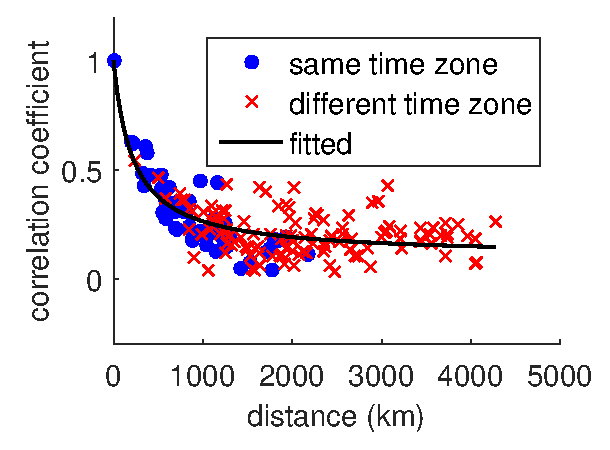
\includegraphics[width=.5\linewidth]{figs/solar_ar_corr_coff}}
	\subfloat[Wind generation]{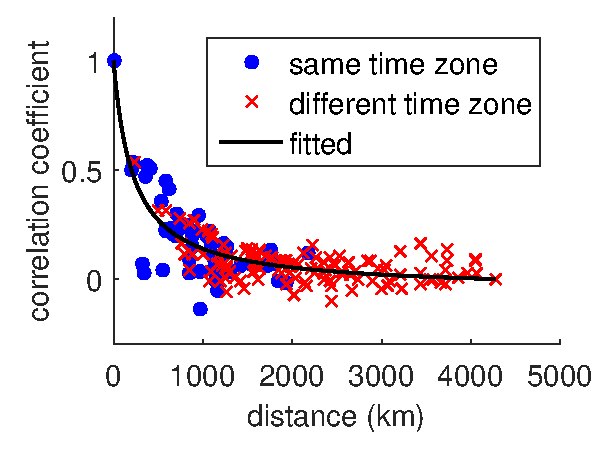
\includegraphics[width=.5\linewidth]{figs/wind_ar_corr_coff}}
	\\
	\subfloat[Electricity prices]{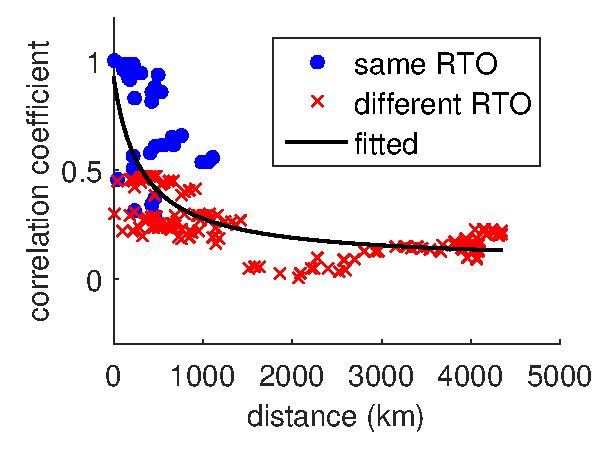
\includegraphics[width=.5\linewidth]{figs/price_ar_corr_coff}}
	\subfloat[Workload]{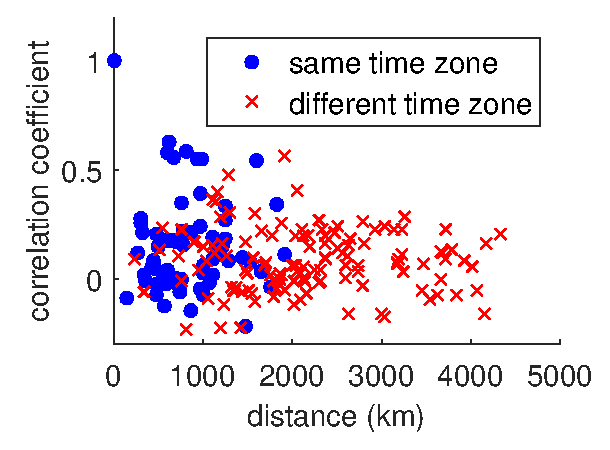
\includegraphics[width=.5\linewidth]{figs/workload_ar_corr_coff}}
	\caption{Correlation coefficients of prediction errors in spatial domain.}
	\label{fig:spaceCorrelation}
\end{figure}

\textbf{How correlated are the prediction errors in spatial domain?} The correlation of prediction errors in the spatial domain is of great interest to cloud providers with geo-distributed data centers. The correlation coefficients of prediction errors using AR with respect to the distance between two locations are shown in Figure \ref{fig:spaceCorrelation}. We classify PV generation, wind generation, and workload into two groups: within the same time zone or different time zones. There are also two groups of electricity prices: within the same RTO or different RTOs. Figure \ref{fig:spaceCorrelation} highlights that both distances \new{and groups can have the great impact on the correlation of prediction errors}\delete{the greater impact on the correlation than the groups have}. The prediction errors of PV and wind generation are strongly correlated (greater than 0.5) within 500 km, weakly correlated (less than 0.5) within 1000 km, and almost independent of each other when more than 1500 km apart. Note that electricity price is more correlated in the spatial domain than PV generation and wind generation due to the fact that some of the prices can be generated by the same RTO. However, the prediction errors of workload are uncorrelated with respect to distances and groups. This is because the workload depends on unpredictable user behavior and the dynamic Internet conditions.


\section{Algorithm Design}
\label{sec:AlgorithmDesign}

The energy procurement system needs algorithms for both energy
procurement in long-term (EP-LT) and geographical load balancing in
real-time (GLB-RT). GLB-RT is a convex optimization problem that can
be solved efficiently in real-time by standard techniques
\cite{liu2011greening}. Thus, we focus on designing algorithms for
energy procurement in the long-term markets. Note that even though
EP-LT is a convex optimization (see
Theorem~\ref{theorem:LT-Convexity}), neither the objective function
nor its gradient admit a closed-form representation, which presents significant challenges. 

In this section,
we design two algorithms, namely, Prediction based Algorithm (PA) and
Stochastic Gradient estimate based Algorithm (SGA) for solving EP-LT.
PA is a heuristic algorithm that requires only the predicted values of renewable generations, workload, and
electricity prices. 
On the other hand, SGA comes with a convergence
guarantee, but requires \emph{samples} from the joint distribution of
renewable generations, workload, and electricity prices. As a result,
SGA can be solved in a \emph{data-driven} manner.

\subsection{Prediction based Algorithm (PA)}
\label{sec:PA}

Prediction based algorithm (PA) relies on the mean
values of renewable generation, workload, and electricity
price. 
% However, obtaining the mean values requires the knowledge of the
% distribution of renewable generation, workload, and electricity
% price.
Fortunately, our data analysis reveals that our prediction errors for
these quantities are approximately zero mean.
%Even though prediction errors are biased, we can simply
%adjust the prediction methods to eliminate the bias. 
%% JK: this contradicts the previous statement.
Thus, the predicted values $\hat{L}^r_j$, $\hat{w}^r_i$, and
$\hat{p}^r_i$ are good estimates of the mean values of renewable
generation, workload, and electricity price.

PA computes the long-term procurement $\Vector{q}^l$ by solving EP-LT
and GLB-RT at the same time, with the random variables $w^r_i$,
$L^r_j$, and $p^r_i$ replaced by their predicted values. Formally, this is done by solving the following deterministic convex optimization problem.
\begin{subequations}
	\begin{align*}
	\text{LT-PA: } & \min_{\mathbf{m}, \Vector{\lambda}, \mathbf{q}^l} \sum_{i=1}^{N} p^l_i q^l_i + \sum_{i=1}^{N} \hat{p}^r_i [m_i - \hat{w}^r_i - q^l_i]_+ \nonumber \\
	&  + \beta  \sum_{i}^{}\sum_{j}^{}h_{ij}(m_i, \lambda_{ij}) \\
	\mbox{subject to } \nonumber \\
	&\text{Constraints \eqref{eq:GLB-RT_c1}, \eqref{eq:GLB-RT_c}--\eqref{eq:GLB-RT_c2}} \\
        &\sum_{i\in N}^{} \lambda_{ij} = \hat{L}^r_j \quad \forall j \in J \\
	&q^l_i \geq 0 \textbf{   } \forall i \in N
	\end{align*}
\end{subequations}
The objective function of LT-PA is similar to that of the EP-LT
without the expectation operation. The constraints over $\Vector{m}$,
$\Vector{\lambda}$, and $\Vector{q}^l$ of LT-PA are identical to those
of GLB-RT and EP-LT. LT-PA is a convex
optimization problem and can be solved efficiently by standard
techniques \cite{boyd2004convex}. 
%% JK -- Removing the adjective `deterministic' from the optimization
%% problem. Note that all our optimizations are determinstic.
Even though PA is a heuristic, our experimental evaluations reveal
that it provides a near-optimal solution in realistic scenarios; see
Section~\ref{sec:caseStudy}.



\subsection{Stochastic Gradient-based Algorithm (SGA)}

Although PA can offer a quick heurictic decision, it is desirable to
have an algorithm that optimally procures electricity in long-term
markets. To this end, we exploit the gradient characterization of the
long-term objective (see Theorem~\ref{theorem:lt_gradient}) to design
a stochastic gradient descent algorithm. The algorithm, namely, SGA,
is summarized in Algorithm \ref{alg:sgea}. The main idea of the
algorithm is to compute a noisy estimate of the gradient of the
long-term objective by averaging the gradient of the (random) total
cost over a finite number of sample paths.
% derived based on results in Section~\ref{sec:dataAnalysis}. 
This noisy gradient is used to perform a stochastic gradient
descent. Stochastic approximation theory can then be used to prove
convergence to the set of optimal solutions, as long as the step-size
sequence is appropriately diminishing \cite{Kushner03}.

%There are two challenges when designing this type of algorithms. First, we have to compute the stochastic gradient of the long-term objective function, which usually does not have a closed form. Fortunately, Theorem \ref{theorem:lt_gradient} provides us the way to compute the stochastic gradient of long term objective. Second, the sequence of step sizes $\{\eta_{\tau}\}_{1 \leq \tau \leq T}$ have to be well designed for the algorithm to converge. $\{\eta_{\tau}\}_{1 \leq \tau \leq T}$ are generated such that $\sum_{ \tau=1 }^{T} \eta _{\tau}= \infty $ and $\sum_{\tau=1}^{T} \eta ^2_{\tau}= \infty $.

\renewcommand{\algorithmicrequire}{\textbf{Input:}}
\renewcommand{\algorithmicensure}{\textbf{Output:}}
\begin{algorithm}
	\caption{Stochastic Gradient based Algorithm (SGA).}
	\label{alg:sgea}
	\begin{algorithmic}
		\REQUIRE Obtain $\Vector{p}^l$ from the $|N|$ long-term electricity markets. \\
		Prepare $\mathbb{S}$ samples of $(\Vector{w}^r,\Vector{L}^r,\Vector{p}^r)$ based on prediction error distributions.
		\ENSURE $q^l_i$ $\forall i \in N$
		\STATE \textit{Initialize:} $q^l_i = {0}$, $\forall i \in N$. 
		\STATE \textit{Step:} $\tau=1$.
		% % \WHILE{$\tau \leq T$}
		\WHILE{true}    
		\FORALL {$k$ such that $1 \leq k \leq \mathbb{S}$}
		\STATE \textit{Solve:} GLB-RT for $k$th sample of $(\Vector{w}^r,\Vector{L}^r,\Vector{p}^r)$ with long-term procurement $\Vector{q}^l$
		\STATE \textit{Obtain:} The Lagrange multipliers $\varrho_i^{(k)}$ corresponding to constraint \eqref{eq:GLB-RT_c3}, $\forall i \in N$
		\ENDFOR    
		\STATE \textit{Compute:} $\hat{\varrho}_i = \frac{1}{\mathbb{S}} \sum_{k = 1}^{\mathbb{S}} \varrho_i^{(k)}$, $\forall i \in N$
		\STATE \textit{Update:} $q^l_i = [q^l_i - \eta_{\tau} (p^l_i - \hat{\varrho}_i)]_{[0,M_i]}$ for $\forall i \in N$. $[z]_{[0,M_i]}$ indicates the projection of $z$ onto
                the set $[0,M_i].$ \STATE \textit{Increase}:
                $\tau=\tau+1$.
		\ENDWHILE
	\end{algorithmic}
\end{algorithm}

% Intuitively, assuming the gradient estimation is accurate enough,
% the algorithm is moving along the direction close to the steepest
% decent one. Therefore, the objective function of EP-LT decreases and
% the gradient $p^l_i-\hat{\varrho}_i$ becomes smaller. Eventually,
% $p^l_i-\hat{\varrho}_i$ approaches 0, and $q^l_i$ converges yielding
% one optimal solution.
%% JK -- I think the explanation preceding the algorothm is
%% sufficient.

We prove that SGA converges to the set of optimal solutions of
EP-LT under the following standard assumption on the step-size
sequence.
\begin{assumption}
	\label{ass:stepsize}
	$\sum_{\tau = 1}^{\infty}(\eta_{\tau}) = \infty $ and
        $\sum_{\tau = 1}^{\infty}(\eta_{\tau})^2 < \infty$.
\end{assumption}
The convergence of SGA is asserted by the following theorem.
\begin{theorem}
	\label{thm:sgea}
	Under Assumption~\ref{ass:stepsize}, almost surely, the iterates
	$\Vector{q}^l$ generated by SGA converge to the set of optimal
	solutions of EP-LT as $\tau \ra \infty.$
\end{theorem}
We give the proof of Theorem~\ref{thm:sgea} in
Appendix~\reference{sec:conv-proof}.


\ignore{ The algorithm first receives electricity price
  $\Vector{p}^l_i$ from long-term markets. It generates all the
  samples of renewable generation, workload, and electricity prices at
  real-time markets from predicted values and prediction error
  distributions as \eqref{eq:predictionErrors}. In the beginning, SGA
  starts with a feasible solution, e.g. $q^l_i=0$. Then, the algorithm
  takes $T$ iterations to approach closer the optimal
  solution. Theoretically, a solution closer to the optimal solution
  can be obtained from using a larger $T$. In practice, $T$ depends on
  the acceptable computational time and the expected accuracy. In each
  iteration $t$, SGA estimates the gradient $\nabla_{q^l_i}(t)$ and
  updates the solution by using
	$$q^l_i(t) = [q^l_i(t-1) - \eta_t \hat{\nabla}_{q^l_i}(t)]_+$$ where $\eta_t$ is the step size such that  And, $[\cdot]_+$ projects $q^l_i(t)$ to the feasible domain.}

      Note that SGA requires samples from the joint distribution of
      $(\Vector{w}^r,\Vector{L}^r,\Vector{p}^r).$ This means that SGA
      can be solved in an entirely data-driven manner, without needing
      to actually model the distributions of workload, renewable
      generation, and electricity price, or the complex
      inter-dependencies between these quantities. This makes it
      particularly suitable in today's `big-data' era. The bottleneck
      of SGA is the computation of the noisy gradient estimate, which
      involves solving $\mathbb{S}$ instances of GLB-RT. Moreover, the
      diminishing step-size sequence implies that SGA requires a large
      number of iterations to compute a near-optimal
      solution. However, it is important to note that since this
      algorithm is only used for long-term procurement, its
      computation time would not be a bottleneck in practice.



\section{Empirical evaluation}
\label{sec:caseStudy}

%In this section, we perform an extensive empirical study evaluating the proposed energy procurement system.
% We first illustrate the fast convergence of SGA to the optimal
% solution in Figure~\ref{fig:convergence}. Then we continue to
% highlight the cost savings by using our system in Figure
% \ref{fig:cost_comparison}. The impacts of renewable energy
% penetration level and prediction errors are also studied.

\textbf{Experimental Setup.} There are 14 data centers in our system. They are located in 10
different states known to have Google data centers: California,
Washington, Oregon, Illinois, Georgia, Virginia, Texas, Florida, North
Carolina, and South Carolina. We merged the data centers in each state
creating 10 logical data centers in our simulation, i.e., $|N|=10$. We
assume that there are one million servers distributed across the ten
logical data centers, which is around half of the
number of servers in Amazon Web Services (AWS)
{\cite{AWSServers}}. The peak power consumption for each server is
300W.
%We set the other parameters based on the baseline case of using the nearest routing technique where the workload is just forwarded to the nearest data centers. 
We consider 40 sources, corresponding to 40 states of the US; the
corresponding workload data is obtained from Akamai Technologies. We
use the model \eqref{eq:delaycost} for capturing the monetary cost of
delay. The average workload is 30\% of the total capacity of the data
centers. The network delays $\pi_{ij}$ are estimated to be
proportional to the distance between sources and data centers
\cite{ATTNetworkLatency}. The average network delay is $22$ ms.
% The average queueing delay is $14.2$ ms. \jk{How do we arrive at
% this number? Does the queueing delay not depend on the algorithm?}
The parameter $\beta$ is estimated according to the fact that 100
ms latency costs 1\% of Amazon in sales \cite{liddle2008amazon}.



To compute the energy costs of the system, we assume that the system
purchases energy in long-term markets and real-time markets for an
hour of operation. The electricity prices in real-time markets are the
industrial electricity prices of each state in May 2010
\cite{eia2015}. Specifically, the mean values of real-time electricity
prices, $\mathbb{E}[p^r_i]$, of the considered states (in cents per
kWh) are as follows: 10.41 in California, 3.73 in Washington, 5.87 in
Oregon, 7.48 in Illinois, 5.86 in Georgia, 6.67 in Virginia 6.44 in
Texas, 8.60 in Florida, 6.03 in North Carolina, and 5.49 in South
Carolina. Since electricity prices in long-term markets are usually
much cheaper than that of the real-time markets, we set the long-term
prices such that the ratio $\frac{\mathbb{E}[p^r_i]}{p^l_i }=2.5$ for
all results, except for Figure~\ref{fig:prices}, where the ratio is
varied.
%We set $\beta$ = 1 throughout the section except Figure
%\ref{fig:betas} where it varies. 


To simulate the uncertainties, the error distributions between 12-13
pm shown in Figure \ref{fig:hourlyDistribution} are used to generate
the samples of renewable energy generation (PV generation and/or wind
generation), workload, and electricity price. The mean absolute errors
(MAE) of prediction errors for PV generation, wind generation,
electricity price, and workload demand are $45\%$, $65\%$, $40\%$, and
$35\%$, respectively. The MAE are varied later to study the impacts of
prediction errors. Wind generation is used as the renewable energy
source by default. The penetration of the renewable energy is fixed at
$50\%$ of the averaged demand. We also vary the penetration of PV and
wind generation to investigate the impacts of the renewable portfolio
and penetration level.

\begin{figure}[!t]
	\centering
	\vspace{-0.2cm}
	\subfloat[Gradient components]{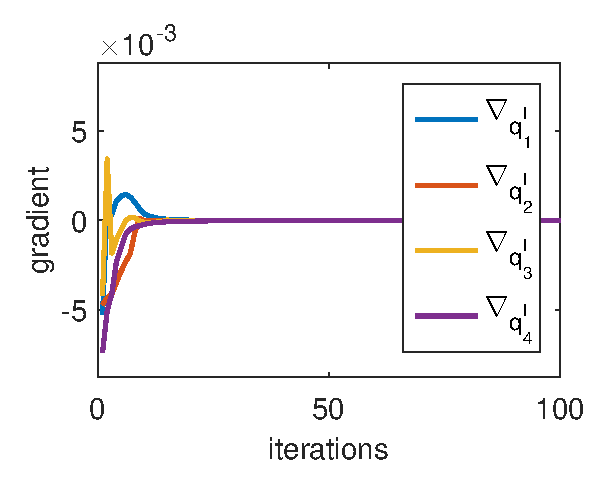
\includegraphics[width=.5\linewidth]{figs/grad_converge}}
	\subfloat[Long-term objective]{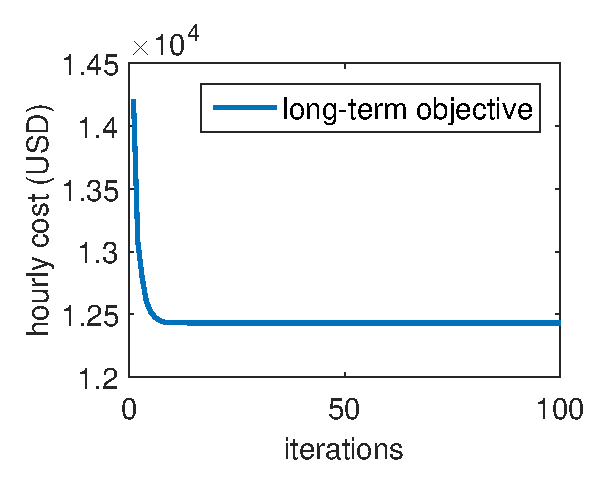
\includegraphics[width=.5\linewidth]{figs/obj_converge}}
	\vspace{-0.2cm}
	\caption{Convergence analysis.}
	\label{fig:convergence}
	\vspace{-0.6cm}
\end{figure}

\textbf{Convergence of SGA.} Although SGA is proved to eventually
converge to the optimal value of EP-LT, the convergence can be slow in
practice. The convergence speed mainly depends on how the step sizes
are set. Stochastic approximation is known to have high computational
complexity due to the large numbers of iterations and samples needed
for each iteration. To reduce the number of iterations, we use the
step size update rule as $\eta_t=\frac{s}{(S+t+1)^\alpha},$ where
$s$ and $S$ are non-negative constants and $ 0.5 < \alpha \leq
1$. This form fulfills the requirement of
Assumption~\ref{ass:stepsize}.
% In general, larger $s$ can enhance the performance in the later
% iterations, but it may cause instability in the early
% iterations. Thus, $S$ is used to prevent the instability.
%% JK: Not sure if this much detail is needed.
To speed up the convergence of algorithm, each gradient component has
its own step-size, and the step-size is updated only if the gradient
component switches from negative to positive or vice versa. Figure
\ref{fig:convergence} illustrates four gradient components (of total
ten) and the long-term objective function updated over iterations. As
shown in the figure, gradient components, and the long-term objective
$F^l(q^l)$ converge very quickly, i.e it is very close to the optimal
value after merely 20 iterations. In general, some gradient components
$\nabla_{q^l_i}$ may converge to positive values. In such cases, the
optimal solution has $q^l_i=0$.

\textbf{Cost savings.} We highlight the benefit of our proposed system
by comparing with the following algorithms.

\textit{No long-term procurement or geographical load balancing (nLTnGLB)}: nLTnGLB does not participate in long-term markets, i.e. $q^l_i = 0$, $\forall i \in N$, and the workload demand are forwarded to the closest data centers, a.k.a., the nearest routing method. We assume that the data centers activate all servers to minimize the queueing delay, i.e. $m_i=M_i$. Though simple, this policy is still widely used in practice.

\textit{Fixed long-term procurement without geographical load balancing (fLTnGLB)}: Cloud providers purchase a fixed amount of electricity ahead. We assume that the long-term procurement is 50\% of workload mean. Like nLTnGLB, it uses the nearest routing method instead of GLB-RT.

\textit{No long-term procurement but with geographical load balancing (nLT)}: In this algorithm, cloud providers do not purchase the energy in long-term markets like nLTnGLB. However, they execute GLB-RT to minimize the total cost in real-time.

\textit{Fixed long-term procurement geographical load balancing (fLT)}: fLT buys a fixed amount of electricity in long-term markets same as fLTnGLB, i.e., 50\% of workload mean. In real-time markets, it executes GLB-RT.

In addition to the baseline algorithms, we compare our algorithms to \textit{Oracle Algorithm (OA)}. OA is an unrealizable algorithm that is given to the absolute performance limit by assuming assumes all realizations of renewable energy, workload, and electricity prices are fully known apriori. Similarly to PA, the problem of long-term procurement can then be solved efficiently. The cost of OA is measured by averaging its output over many realizations.

\desc{The benefits of the proposed system}

\begin{figure}[!ht]    
	\centering
	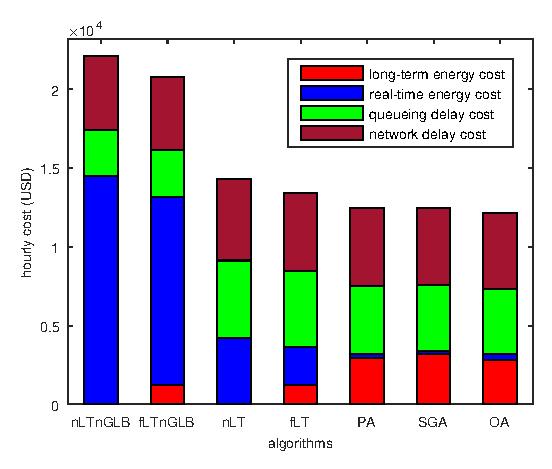
\includegraphics[width=.95\linewidth]{figs/cost_comparison}
	\vspace{-0.3cm}
	\caption{Cost comparison when $\beta=1$ and 50 \% renewable penetration. The proposed algorithms PA and SGA  are very close to the lower bound, OA and outperform the traditional methods up to 44\%.}
	\label{fig:cost_comparison}
	\vspace{-0.5cm}
\end{figure}

Figure \ref{fig:cost_comparison} compares the cost performance among our proposed algorithms and the traditional algorithms. The figure highlights that our proposed algorithms PA and SGA save up to 44\% compared to other simpler algorithms, and are comparable to the oracle algorithm (OA), the impractical lower bound. It also shows the significant benefits for cloud providers to participate long-term markets. Surprisingly, the performance of PA is very close to that of the SGA.

%\todo{read the paper A Control Theorist’s Perspective on Dynamic Competitive Equilibria in Electricity Markets by Wang et al. to see whether it can explain this observation.}

%\new{A Control Theorist’s Perspective on Dynamic Competitive Equilibria in Electricity Markets CANNOT be used to explain the observation.
%	a) The paper models the competitive equilibrium between customers and suppliers to explain that why the electricity prices are volatile. It has nothing to do with our model.
%	b) In our paper, the real-time electricity prices can be volatile or not and this property of electricity prices have nothing to to with the very good performance of PA.}

\diff{\textbf{Why do our proposed algorithms perform so well?} The intuition behind the small performance gaps between PA, SGA and OA is the compensation of GLB-RT at real-time markets. In particular, GLB-RT can utilize the available renewable energy and cheap electricity to partially compensates for performance gap caused by the prediction errors in long-term. More interestingly, PA and SGA are noticeably aggressive in long-term markets as in Figure \ref{fig:cost_comparison}. In addition, PA and SGA are even more aggressive than OA. In fact, Lemma \ref{theorem:RealTimeOptimalDemand} allows PA, SGA, and OA to purchase a lot of electricity in long-term markets, because the over-provisioned energy can be used up to reduce queuing delay in real-time. Thus, there is the trade-off between the energy costs and delay costs that helps our proposed methods become close to OA.}

\begin{figure}[!h]    
	\centering
	\vspace{-0.3cm}
	\subfloat[$\beta=0$]{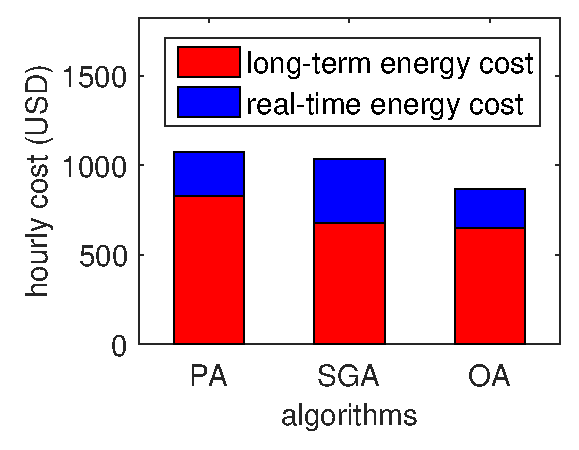
\includegraphics[width=.5\linewidth]{figs/cost_comparison_beta_0} 
		\label{fig:beta_0}}
	\subfloat[Vary $\beta$]{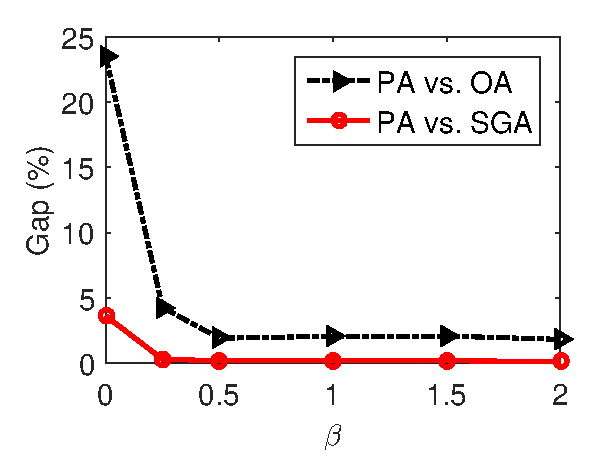
\includegraphics[width=.5\linewidth]{figs/vary_beta}
		\label{fig:vary_beta}}    
	\caption{The impact of delay on the proposed algorithms.}
	\label{fig:betas}
	\vspace{-0.3cm}
\end{figure}

\diff{\emph{How does the trade-off between energy costs and delay costs benefit our proposed algorithms?}
To answer this question, we vary the constant factor $\beta$ that weighs the delay costs relative to energy costs.
When $\beta=0$, i.e., the delay costs are ignored, the cost breakdown are shown in Figure \ref{fig:beta_0}. The performance gap between PA
and OA is 24\% that is much larger than the 2\% gap in Figure \ref{fig:cost_comparison} ($\beta=1$).
In this setting, SGA outperforms PA by 4\%. We observe that PA is more
aggressive compared to SGA in long-term procurement. Figure
\ref{fig:vary_beta} shows the performance gaps of PA versus OA and PA
versus SGA with varying $\beta.$ In this figure, the x-axis shows a
scaled $\beta,$ where a value of 1 corresponds to the default value.
We note that the performance gaps are significant when $\beta$ is
small ($<0.25$). However, the gaps are very small when $\beta$ is
relatively large ($\geq 0.5$).
}
%To show that GLB helps PA to perform well, we carry out another experiment assuming that there is only one single data center in our system. The performance comparison is in Figure \ref{fig:single_dc}

%SGA is proved to have optimal cost saving and robust to any prediction error correlations and a much wider range of objective functions. Therefore, it is usually worth using SGA for large-scale geo-distributed data center systems which cost billions of dollars a year.


\diff{\textbf{Sensitivity Analysis}. The capability of our proposed algorithms depends on multiple impact factors, such as the ratio of real-time price to long-term price, renewable penetration rates, and prediction errors.}
%Hence, it is necessary to study the impact of these impact factors on the proposed algorithms.

\begin{figure}[!ht]    
	\centering
	\vspace{-0.5cm}
	\subfloat[PA vs. OA]{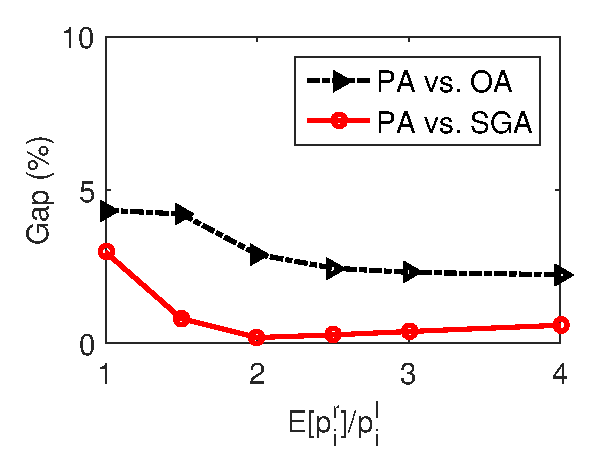
\includegraphics[width=.5\linewidth]{figs/vary_p_l_ratio}
		\label{fig:vary_p_l_ratio}}    
	\subfloat[Long term procurement]{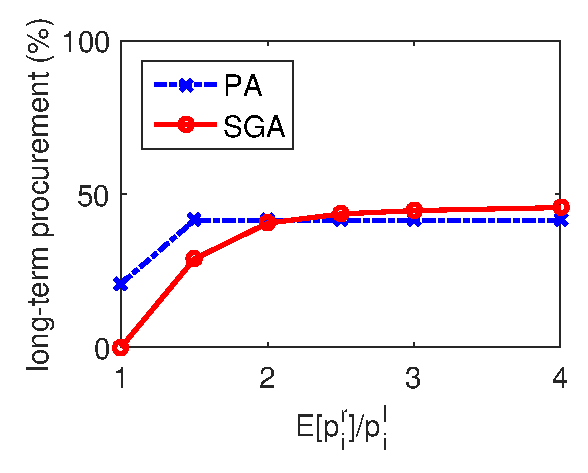
\includegraphics[width=.5\linewidth]{figs/vary_p_l_long_term_markets}
		\label{fig:vary_p_l_long_term_markets}}
	\vspace{-0.2cm}
	\caption{The impacts of long-term prices on the proposed algorithms. The gaps between the proposed algorithms and OA are small at various ratios of real-time prices to long-term prices.}
	\label{fig:prices}
	\vspace{-0.3cm}
\end{figure}

\emph{Impact of the ratio of real-time price to long-term price.} We carry out another study that quantifies the impact of the ratio of real-time prices to the long-term prices on our proposed algorithms as in Figure {\ref{fig:prices}}. In this experiment, the long term prices are fixed, and we scale the real-time prices. Figure {\ref{fig:vary_p_l_ratio}} shows the performance gaps of PA versus SGA and PA versus OA. In general, the gaps are small whatever the ratio is. Figure {\ref{fig:vary_p_l_long_term_markets}} illustrates the behaviors of PA and SGA in long-term markets. SGA is more conservative than PA when the ratio is small ($<2$). When the real-time prices are as cheap as the long-term prices, being more aggressive in long-term actually results in higher financial risk to the cloud providers. In contrast, SGA is more aggressive in long-term markets as the ratio becomes larger than 2.

\emph{Impact of renewable energy.} Renewable energy has been increasingly used to power data centers. Hence, we investigate the impacts of renewable energy integration on our energy procurement system. We scale the penetration levels of renewable energy from $5\%$ to $95\%$ of the total demand. We consider PV generation and wind generation as two main sources of renewable energy.

\begin{figure}[!ht]    
	\centering
	\vspace{-0.3cm}
	\subfloat[PV penetration]{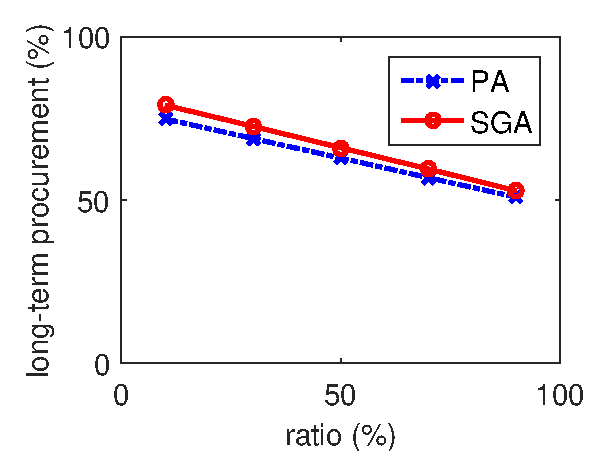
\includegraphics[width=.5\linewidth]{figs/solar_impact2}}
	\subfloat[Wind penetration]{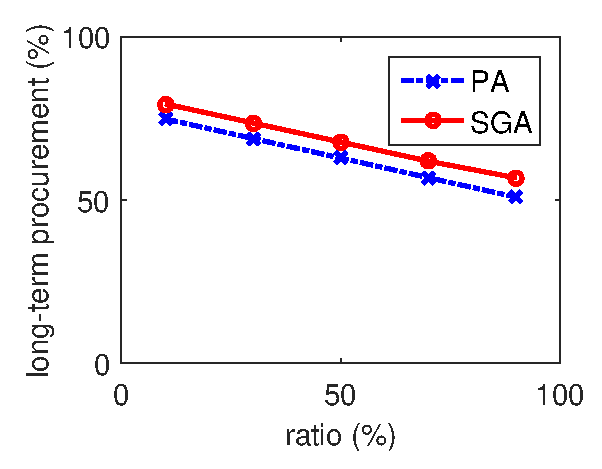
\includegraphics[width=.5\linewidth]{figs/wind_impact2}} 
	\vspace{-0.2cm}
	\caption{Impacts of renewable energy penetration levels on long-term energy procurement. SGA becomes less aggressive in the PV generation case than the wind generation case compared to PA.}
	\label{fig:renewableImpactLTEnergy}
	\vspace{-0.2cm}
\end{figure}

The impacts of renewable energy on the behaviors of PA and SGA are shown in Figure \ref{fig:renewableImpactLTEnergy}. Here, the x-axis represents the penetration levels of renewable energy, and the y-axis is the ratio (\%) of total electricity purchased in long-term markets. PA performs similarly in both cases because it is only based on the predicted values. However, SGA is closer to PA in the PV generation case as the penetration of renewable energy increases, yet becomes more aggressive than PA in the wind generation case. The reason lies in the error distributions in Figure \ref{fig:hourlyDistribution}. While the prediction errors of PV generation are concentrated on two peaks, the prediction errors of wind generation are centered around only one peak (around $-80\%$). 

%It means that wind generation allows SGA to find an optimal solution corresponding to the unique peak, but SGA has to find an optimal solution corresponding to a point between the two peaks.

%\subsection{How can the long-term forecaster impacts on SGA?} 

\emph{Impact of prediction errors.} So far, we have worked with the
empirical (or `real') prediction error distributions. We now study the
dependence of the distribution of prediction errors on the performance
of our procurement system.
%We obtained the prediction errors from AR methods. However, different prediction methods may give different error distributions. Furthermore, as the prediction range varies from days to years, the MAEs of prediction also increases. Thus, we continue to study the impacts of error distributions and MAEs.

\begin{figure}[!h]    
	\centering
	\vspace{-0.5cm}
	\subfloat[Error distributions ]{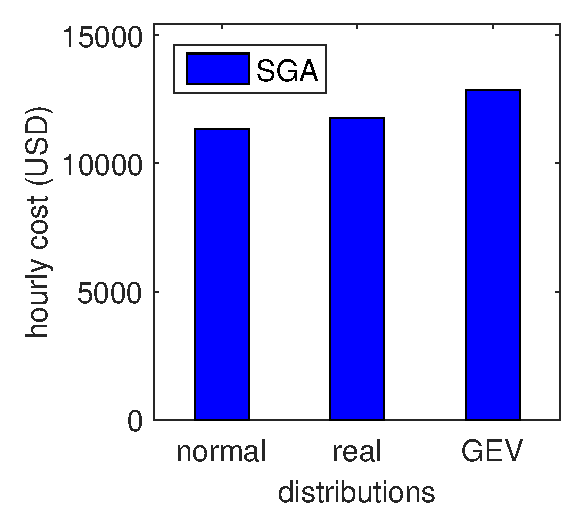
\includegraphics[width=.5\linewidth]{figs/distribution_impact}
		\label{fig:impactOfErrorDistribution_a}}
	\subfloat[Prediction errors ]{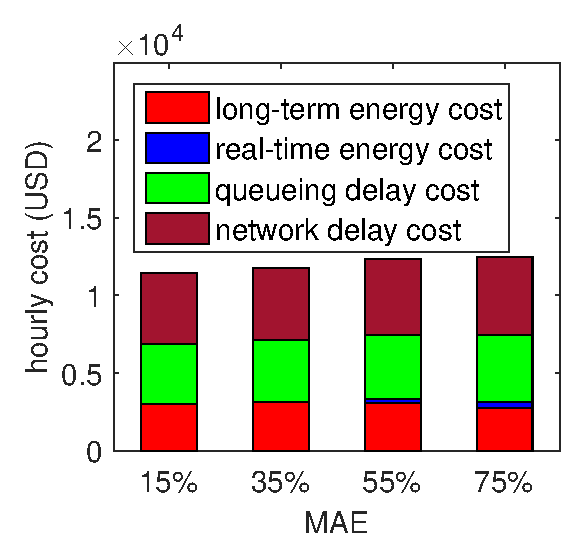
\includegraphics[width=.5\linewidth]{figs/rmse_impact}
		\label{fig:impactOfErrorDistribution_b}}  
	\vspace{-0.2cm}  
	\caption{Impacts of predictions on cost performance.}
	\label{fig:impactOfErrorDistribution}
	\vspace{-0.2cm}
\end{figure}

Figure \ref{fig:impactOfErrorDistribution_a} presents the cost of SGA under three different error distributions, i.e. normal, `real, and generalized extreme value (GEV)~\cite{corcoran2002modelling}. The normal distribution is symmetric around its mean. The GEV distribution is asymmetric and widely used in risk management and finance. We also consider the distribution of AR prediction errors as the `real' distribution. The MAEs of each are set at 35\% for fair comparison. Figure \ref{fig:impactOfErrorDistribution_a} shows that the cost using normal distribution is the best among three error distributions while GEV is the worst. %Similarly to previous case studies, PA also achieves very close performance to SGA. 

Figure \ref{fig:impactOfErrorDistribution_b} shows the cost of SGA with respect to different MAEs of `real' distribution.  As the prediction errors increase, the real-time cost (real-time energy cost and delay cost) increase to compensate for the mis-provisioning in long-term markets. Furthermore, the total cost increases by 10\% as the prediction errors increase from 15\% to 75\%. 


\section{Concluding remarks}

In this paper, we present a systematic study of optimal energy procurement systems for geo-distributed data centers that utilize multi-timescale electricity markets. The contributions of this paper are three-fold: (i) designing algorithms for long-term electricity procurement in multi-timescale markets; (ii) analyzing  long-term prediction errors using real-world traces; and (iii)  empirically evaluating the benefits of our proposed procurement systems. In particular, we proposed two algorithms, PA and SGA, both of which save up to 44\% of the energy procurement cost compared to traditional algorithms that do not use long-term markets or geographical load balancing.  While SGA provably converges to an optimal solution, PA surprisingly achieves a cost that is nearly optimal with much less computing effort. 

There are a number of interesting directions for future research that can be motivated by our work. For example, generalizing our model to include more complicated forward contracts that procure energy that can be used over multiple time-slots is also another challenging problem. Integrating storage capabilities, e.g., batteries and/or thermal storage, into the energy procurement optimization of multi-timescale markets is another challenging direction. The further research on how to optimally utilize multi-timescale markets will have high potential to greatly impact the cost efficiency of Internet-scale services.

\phantomsection
\label{EndOfPaper}
\section{Acknowledgements}
This research is supported by NSF grants CNS-1464388, CNS-1617698, CNS-1730128, CNS-1717588, and CNS-1413998. This research was partially funded by the MSIP, Korea, under the ``ICT Consilience Creative Program'' (IITP-2015-R0346-15-1007) supervised by the IITP and under the ``Basic Science Research Program'' (NRF-2015R1C1A1A01053788) through the NRF, Korea.


%\input{samplebody-conf}

{
\bibliographystyle{ACM-Reference-Format}
\bibliography{bib/sigproc}
}
%\appendix

\section{Proofs for Section 3}
%\nhattan{I updated A.1, A.2, A.3}

\subsection{Proof of Theorem \ref{theorem:LT-Convexity}}
\label{proof:convexity}

To prove Theorem~\ref{theorem:LT-Convexity}, we first show that the
real-time objective is jointly convex with respect to
$(\Vector{q}^l,\Vector{m},\Vector{\lambda}).$
\begin{lemma}
	\label{lemma:rt-convex}
	$\tilde{F}^r$ as defined in \eqref{eq:rt-obj2} is jointly
        convex with respect to
        $(\Vector{q}^l,\Vector{m},\Vector{\lambda})$ over
        $\mathbb{R}^N_+ \times C(L^r).$
\end{lemma}
\begin{proof}
	We rewrite
	\begin{eqnarray}
          \tilde{F}^r(\Vector{q}^l,\Vector{m},\Vector{\lambda},\Vector{p}^r,\Vector{w}^r) = 
          \sum_{i=1}^{N} p^l_i [m_i-w^r_i-q^l_i]_+ \nonumber \\
          + \sum_{i=1}^{N}\sum_{j=1}^{J} \lambda_{ij} h_{ij}(m_i,\lambda_i).
	\end{eqnarray}
	
        %	$\sum_{i=1}^{N} p^l_i q^l_i$ and
        % $\sum_{i=1}^{N}\sum_{j=1}^{J} \lambda_{ji} \pi_{ij}$ are
        % convex.
	
	Since $m_i-w^r_i-q^l_i$ is an affine function, and $[\cdot]_+$
        is convex and non-decreasing, $\sum_{i=1}^{N} p^l_i
        [m_i-w^r_i-q^l_i]_+$ is jointly convex with respect to
        $(\Vector{q}^l,\Vector{m}).$

	
	Since $\lambda_{ij} h_{ij}(m_i,\lambda_i)$ is jointly convex with respect to $(\Vector{m},\Vector{\lambda})$ , 
        $\tilde{F}^r$ is jointly convex with respect to
        $(\Vector{q}^l,\Vector{m},\Vector{\lambda})$ because the
        summation of convex functions are convex.
\end{proof}

\begin{proof}[of Theorem~\ref{theorem:LT-Convexity}]
  From Lemma~\ref{lemma:rt-convex}, we know that the real time
  objective function
  $\tilde{F}^r(\Vector{q}^l,\Vector{m},\Vector{\lambda},\Vector{p}^r,\Vector{w}^r)$
  is jointly convex with respect to
  $(\Vector{q}^l,\Vector{m},\Vector{\lambda}).$ It then follows
  that $$F^{*r}(\Vector{q}^l,\Vector{p}^r, \Vector{L}^r, \Vector{w}^r)
  = \min_{(\Vector{m},\Vector{\lambda}) \in C(L^r)}
  \tilde{F}^r(\Vector{q}^l,\Vector{m},\Vector{\lambda},\Vector{p}^r,\Vector{w}^r)$$
  is convex with respect to $\Vector{q}^l$ (see
  \cite{boyd2004convex}). Finally, since the expectation operation
  preserves convexity, we conclude that $F^l(\Vector{q}^l)$ is convex
  with respect to $\Vector{q}^l.$
\end{proof}


\subsection{Proof of Theorem~\ref{theorem:lt_gradient}}
\label{proof:lt_grad}

This section is devoted to the proof of
Theorem~\ref{theorem:lt_gradient}.  \ignore{Let us
  define $$F^{*r}(q^l,p^r,L^r,w^r):= \min_{(m,\Lambda) \in C(L^r)}
  F^r(q^l,m,\Lambda,p^r,w^r).$$ With this notation, note
  that $$\hat{F}^l(q^l,p^r,L^r,w^r) = \sum_{i \in N} p^l_i q^l_i +
  F^{*r}(q^l,p^r,L^r,w^r).$$} To prove
Theorem~\ref{theorem:lt_gradient}, it suffices to show that
\begin{equation}
  \label{eq:lt_gradient_1}
  \begin{array}{rl}
    \frac{\partial \Exp{F^{*r}(\Vector{q}^l,\Vector{p}^r,\Vector{L}^r,\Vector{w}^r)}}{\partial q^l_i} &= \Exp{\frac{\partial F^{*r}(\Vector{q}^l,\Vector{p}^r,\Vector{L}^r,\Vector{w}^r)}{\partial q^l_i}}\\
  &=
  -\Exp{\varrho_i(\Vector{q}^l,\Vector{p}^r,\Vector{L}^r,\Vector{w}^r)}.      
  \end{array}
\end{equation}
The first step is to prove that the Lagrange multiplier of GLB-RT
corresponding to the constraint \eqref{eq:GLB-RT_c3} is unique.
\ignore{
\jk{Add assumption earlier that wind follows a continuous
  distribution. We need this for the following reason: The proof of
  uniqueness of the Lagrange multiplier requires that the constraint
  $m_i \geq 0$ is not binding. This becomes problematic when the
  optimal $\lambda_i = 0,$ in which case the optimal $m_i$ becomes
  ill-posed. One (not very elegant) fix to this is to assume $w^r$ is
  continuous. This implies that $w^r_i > 0$ with probability 1, which
  implies that we may take $m_i> 0$ with probability 1.}}
\begin{lemma}
  \label{lemma:lt_grad_1}
  With probability 1, GLB-RT has a unique Lagrange multiplier, denoted
  $\varrho_i(\Vector{q}^l,\Vector{p}^r,\Vector{L}^r,\Vector{w}^r),$
  corresponding to the constraint \eqref{eq:GLB-RT_c3}.
\end{lemma}
\begin{proof}
  In this proof, for notational simplicity, we suppress the dependence
  of the primal and dual solutions of GLB-RT on
  $(\Vector{q}^l,\Vector{p}^r,\Vector{L}^r,\Vector{w}^r).$ Consider a
  primal solution of GLB-RT
  $(\Vector{q}^r,\Vector{m},\Vector{\lambda})$ with $\Vector{m} > 0.$
  Such a solution exists with probability 1, since $\Vector{w}^r > 0$
  with probability 1.

  Now any dual solution must satisfy the KKT conditions. This implies
  the following conditions. (Since the constraint $\lambda_i \leq m_i
  \mu_i$ is never binding, the corresponding Lagrange multiplier
  $\sigma_i = 0$ and does not feature in the following.)
\begin{align}
  \label{eq:kkt_1}
  & \frac{\partial}{\partial m_i} \sum_{i=1}^{N}\sum_{j=1}^{J} \lambda_{ij} h_{ij}(m_i,\lambda_i) + \bar{\omega}_i - \underbar{$\omega$}_i + \varrho_i = 0\\%+ \gamma_ie_0= 0 \\
  \label{eq:kkt_2}
  &\bar{\omega}_i(m_i - M_i) = 0;\  \bar{\omega}_i \geq 0, m_i \leq M_i \\
  \label{eq:kkt_3}
  &\underbar{$\omega$}_i m_i = 0; \ \underbar{$\omega$}_i \geq 0, m_i \geq 0 \\
  \label{eq:kkt_4}
  &p_i^r - \kappa_i - \varrho_i= 0 \\
  \label{eq:kkt_5}
  &\kappa_i q^r_i = 0; \kappa_i \geq 0, q^r_i \geq 0 \\
  \label{eq:kkt_6}
  &\varrho_i(-q^r_i + m_i - w^r_i - q^l_i)  = 0; \\
  \label{eq:kkt_7}
  &\varrho_i \geq 0, q^r_i \geq m_i - w^r_i - q^l_i
\end{align}

We now argue that $\varrho_i$ is unique for all $i.$ Consider the
following two cases.

\noindent {\bf Case 1:} $w^r_i + q^l_i > M_i.$ In this case, it
follows that $m_i <w^r_i + q^l_i + q^r_i.$ Using \eqref{eq:kkt_6}, we
conclude that $\varrho_i = 0.$

\noindent {\bf Case 2:} $w^r_i + q^l_i < M_i.$ Here we consider two
sub-cases. \\
{\bf Case 2a:} $m_i = M_i.$ In this case, it follows that $q^r_i > 0,$
which implies that $\kappa_i = 0$ (by \eqref{eq:kkt_5}). Thus, we
have, using \eqref{eq:kkt_4}, that $\varrho_i = p^r_i.$\\
{\bf Case 2b:} $m_i < M_i.$ In this case, since $m_i \in (0,M_i),$ we
have $\bar{\omega}_i = \underbar{$\omega$}_i = 0$ 
(by \eqref{eq:kkt_2}
and \eqref{eq:kkt_3}). Thus, from \eqref{eq:kkt_1}, we
have 
\begin{equation}
\label{eq:der_closed_form}
\varrho_i = -\frac{\partial}{\partial m_i} \sum_{i=1}^{N}\sum_{j=1}^{J} \lambda_{ij} h_{ij}(m_i,\lambda_i). %-\gamma_i.
\end{equation}
%Because it is assumed that $d^r_i=D_i$ only if all $M_i$ servers are active and run at their peak power and in Case 2b $m_i < M_i$, $\gamma_i=0$.

Since the event $w^r_i + q^l_i = M_i$ 
has zero probability, we may
ignore this case. This completes the proof.
%The idea is that if the Lagrange multiplier $\varrho_i(\Vector{q}^l,\Vector{p}^r,\Vector{L}^r,\Vector{w}^r)$ is not unique, it cannot be obtained by optimizing GLB-RT.
%
%Assuming that $\frac{\partial F^{*r}(q^l,p^r,L^r,w^r)}{\partial q^l_i} = \varrho_i(\Vector{q}^l,\Vector{p}^r,\Vector{L}^r,\Vector{w}^r)$ is not unique, there exist two optimal solutions $\underline{q}^{l}_i$ and $\bar{q}^l_i$ at data center $i$ such that 
%$$\frac{\partial \Exp{F^{*r}(.)}}{\partial \underline{q}^{l}_i} \neq \frac{\partial \Exp{F^{*r}(.)}}{\partial \bar{q}^{l}_i} $$
%
%Since $F^{*r}(.)$ is convex over $q^l_i$, we have ${q}^{\gamma}_i = \chi \underline{q}^{l}_i + (1-\gamma) \bar{q}^{l}_i$ with $0<\gamma<1$ such that
%$F^{*r}({q}^{\gamma}_i) \leq F^{*r}(\bar{q}^{l}_i) + (1-\gamma)F^{*r}(\underline{q}^{l}_i)$. 
%$F^{*r}(\bar{q}^{l}_i)$ and $F^{*r}(\bar{q}^{l}_i)$ are both optimal, thus  
%$$F^{*r}({q}^{\gamma}_i) = F^{*r}(\bar{q}^{l}_i) + (1-\gamma)F^{*r}(\underline{q}^{l}_i)$$ which means that $F^{*r}$ is linear on $[\underline{q}^{l}_i, \bar{q}^l_i]$. Hence, its gradients on $[\underline{q}^{l}_i, \bar{q}^l_i]$ are constant that contradicts the assumption.
\end{proof}

Given Lemma~\ref{lemma:lt_grad_1}, it follows from standard
sensitivity analysis in convex optimization (see Section~6.5.3 and
~6.5.4 in \cite{Bertsekas03}) that 
\begin{equation}
  \label{eq:grad_lt}
  \frac{\partial
    F^{*r}(\Vector{q}^l,\Vector{p}^r,\Vector{L}^r,\Vector{w}^r)}
  {\partial q^l_i} =-
  \varrho_i(\Vector{q}^l,\Vector{p}^r,\Vector{L}^r,\Vector{w}^r).  
\end{equation}
This proves the second equality in \eqref{eq:lt_gradient_1}. Thus, to
complete the proof of Theorem~\ref{theorem:lt_gradient}, it only
remains to justify the interchange of the partial derivative and the
expectation in the first equality. We justify this interchange by
invoking the dominated convergence theorem as follows.

Let $e_i$ denote a column vector in $\mathbb{R}^N,$ with 1 in the
$i$th entry and 0 elsewhere.
\begin{lemma}
  \label{lemma:lt_grad_2}
  For any $\delta \neq 0$ and $i \in N,$
  \begin{equation*}
    \left|\frac{F^{*r}(\Vector{q}^l + \delta e_i,\Vector{p}^r,\Vector{L}^r,\Vector{w}^r) - 
        F^{*r}(\Vector{q}^l,\Vector{p}^r,\Vector{L}^r,\Vector{w}^r)}{\delta}\right| \leq p^r_i.
  \end{equation*}  
\end{lemma}
\begin{proof}
  It is easy to see
  that $$F^{*r}(\Vector{q}^l,\Vector{p}^r,\Vector{L}^r,\Vector{w}^r)
  \leq \delta p^r_i + F^{*r}(\Vector{q}^l + \delta
  e_i,\Vector{p}^r,\Vector{L}^r,\Vector{w}^r).$$ The statement of
  Lemma~\ref{lemma:lt_grad_2} follows from the fact that
  the function $F^{*r}(\Vector{q}^l + \delta
  e_i,\Vector{p}^r,\Vector{L}^r,\Vector{w}^r)$ is non-increasing with
  respect to $\delta.$
\end{proof}

Since $\Exp{p^r_i} < \infty,$ it follows from the dominated
convergence theorem that 
\begin{align*}
  &\Exp{\lim_{\delta \ra 0} \frac{F^{*r}(\Vector{q}^l + \delta
      e_i,\Vector{p}^r,\Vector{L}^r,\Vector{w}^r) -
      F^{*r}(\Vector{q}^l,\Vector{p}^r,\Vector{L}^r,\Vector{w}^r)}{\delta}} \\
  &\quad =\lim_{\delta \ra 0} \frac{\Exp{F^{*r}(\Vector{q}^l + \delta
      e_i,\Vector{p}^r,\Vector{L}^r,\Vector{w}^r)} -
    \Exp{F^{*r}(\Vector{q}^l,\Vector{p}^r,\Vector{L}^r,\Vector{w}^r)}}{\delta}.
\end{align*}
This proves the first equality in \eqref{eq:lt_gradient_1}, and
completes the proof of the theorem.


\subsection{Proof of Lemma~\ref{theorem:RealTimeOptimalDemand}}
\label{proof:RealTimeOptimalDemand}

 We assume there an optimal solution $S$ such that $\lambda_i>0$ and $0 < m_i < w^r_i + q^l_i$. $\lambda_i=0$ or $m_i = 0$ is not ignored because it is equivalent to shutting down data center $i$. Here, $\underbar{$\omega$}_i=\varrho_i = 0$.
 
 If $w^r_i + q^l_i < M_i$ and $m_i < w^r_i + q^l_i$, $\bar{\omega}_i = 0$. $\bar{\omega}_i = \underbar{$\omega$}_i=\varrho_i = 0$ results in $\lambda_i/m_i$ becomes zero as \eqref{eq:kkt_1}. $\lambda_i=0$ or $m_i = \infty$ contradicts the assumption. So, $m_i \geq w^r_i+q^l_i$ if $w^r_i + q^l_i < M_i$. 
 
 If $w^r_i + q^l_i \geq M_i$, we assume that $m_i < M_i$. $\bar{\omega}_i = \underbar{$\omega$}_i=\varrho_i = 0$ again leads to the contradiction to the assumption. So, $m_i=M_i$ if $w^r_i + q^l_i \geq M_i$.

\section{Convergence of SGA}
\label{sec:conv-proof}

This section is devoted to the proof of Theorem~\ref{thm:sgea}.
Invoking Theorem~2.1 in \cite{Kushner03}, the almost sure convergence
of the iterates of SGA to the set of optimal solutions of EP-LT holds
if the following two conditions are satisfied.
  \begin{enumerate}
  \item $\nabla F^l:\R^N_+ \ra \R^N$ is continuous.
  \item $ \sup_{q^l \in \R^N_+}
    \Exp{(\varrho_i(\Vector{q}^l,\Vector{p}^r,\Vector{L}^r,\Vector{w}^r))^2}
    < \infty.$
  \end{enumerate}
  Condition~(1) above holds since the gradient of a differentiable
  convex function is \delete{convex} \new{continuous}; see Theorem 25.5 in
  \cite{Rockafellar70}. Condition~(2) holds since $$
  \varrho_i(\Vector{q}^l,\Vector{p}^r,\Vector{L}^r,\Vector{w}^r) \leq
  p^r_i$$ (see \eqref{eq:grad_lt} and
  Lemma~\ref{lemma:lt_grad_2}). This completes the proof.



% \begin{lemma}
%   \label{lemma:sgea-3}
%   The iterates $q^l(n)$ generated by the SGEA algorithm are almost
%   surely bounded.
% \end{lemma}
% \jk{This is also easy. If any component $i$ of $q^l_i$ exceeds
% $M_i$, then
% $\varrho_i(\Vector{q}^l,\Vector{p}^r,\Vector{L}^r,\Vector{w}^r) = 0$
% for any $(\Vector{p}^r,\Vector{L}^r,\Vector{w}^r),$ implying the
% algorithm will necessarily decrease $q^l_i.$}

%\section{Figures for predictability analysis}
%
%\subsection{Electricity prices}
%
%\begin{figure}[!t]
%	\centering
%	\subfloat[Houton, Texas]{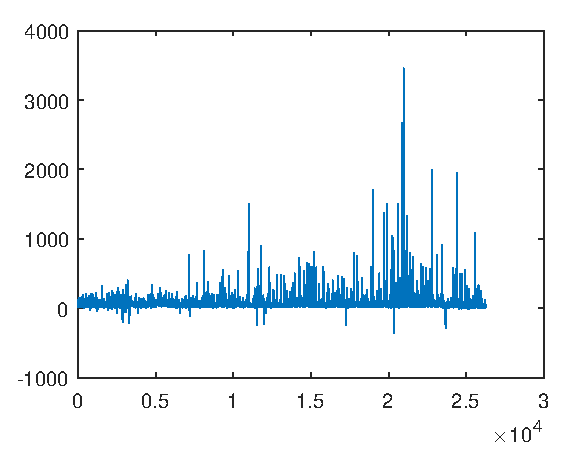
\includegraphics[width=.5\linewidth]{figs2/electricity_prices_TX}}
%	\subfloat[Ohio]{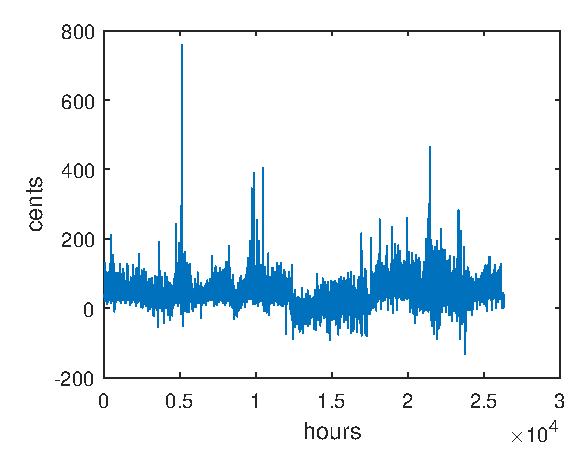
\includegraphics[width=.5\linewidth]{figs2/electricity_prices_OH}}
%	\caption{Electricity prices.}
%	\label{fig:electricityPrices}
%\end{figure}

 
\input{scripts/Appendices3} 

\section{Performance 17 review summary}

The main optimization problem (Equation (3)) is presented assuming that the parameters and the forecast errors are stationary. In practice (as remarked in Section 5 of the
paper), this is not the case : there is seasonality, correlation between errors or hidden effect. I would the results change in this case?  SGA would not be optimal under non-stationary error.
\nhattan{I think our solution is optimal even if it is not stationary as we are searching for the optimal one of the sample space that contains all possible realizations.}

Some workload cannot simply be delayed, so it cannot be simply translated into a cost. The amount of workload that can be delayed, or that have tight delay constraint, might be large and this might have an impact on the performance of the proposed algorithms and on the conclusions and discussions presented in the paper. 
\nhattan{Agree. I still do not know whether our method works if we classify 2 types of workloads: delay tolerant and non-delay tolerant. However, it is beyond this paper scope.}

several data centers work on a model that consists in partinioning the resources and assigning them to tasks. Hence, models based on processor-sharing or single-server queuing might be suited for describing the data-center, especially if the overall data center is considered (and not simply one of the servers). \nhattan{The model would be too detailed (perhaps not general) if we go deeply to this topic. In addition, it will not change the message of the paper.}  

The result in (7) (i.e., optimal solution for energy procurement) directly depends on the assumptions about the delay cost. Hence, I think this point is really critical and should be carefully considered.
Also, it is likely that the cost of additional delay, in real systems, can be large (the provider is probably not that willing to decrease QoS for cost reduction). \nhattan{If the delay is so critical, we will have less flexibility on GLB-RT. Obviously, long-term markets do not offer much benefit when the delay cost is dominant. Furthermore, GLB-RT will play more important role in minimizing the total cost. We already have some flavor in Figure \ref{fig:betas}. So, it is not necessary to add this.}



\end{document}
